\documentclass[twocolumn,10pt]{article}

\usepackage[utf8]{inputenc}
\usepackage[T1]{fontenc}
\usepackage{amsmath,amssymb,amsthm}
\usepackage{graphicx}
\usepackage{xcolor}
\usepackage{hyperref}
\usepackage{booktabs}
\usepackage{caption}
\usepackage{subcaption}
\usepackage{float}
\usepackage{braket}
\usepackage{multirow}
\usepackage{array}
\usepackage{mdframed}
\usepackage{tikz}
\usepackage{orcidlink}
\usetikzlibrary{arrows.meta,positioning,calc,decorations.pathreplacing,patterns}

\hypersetup{
    colorlinks=true,
    linkcolor=blue,
    citecolor=blue,
    urlcolor=blue
}

\renewcommand{\hbar}{\hslash}
\newcommand{\kB}{k_{\text{B}}}
\newcommand{\Tr}{\text{Tr}}
\newcommand{\meV}{\text{~meV}}
\newcommand{\ps}{\text{~ps}}
\newcommand{\fs}{\text{~fs}}
\newcommand{\mus}{\text{~}\mu\text{s}}
\newcommand{\Hz}{\text{~Hz}}
\newcommand{\THz}{\text{~THz}}
\newcommand{\DFS}{\text{DFS}}
\newcommand{\ENAQT}{\text{ENAQT}}

\newtheorem{proposition}{Proposition}
\newtheorem{corollary}{Corollary}
\newtheorem{definition}{Definition}
\newtheorem{remark}{Remark}
\newtheorem{theorem}{Theorem}
\newtheorem{lemma}{Lemma}

\title{\textbf{Quantum coherence in microtubule proteins: theoretical
constraints, non-equilibrium mechanisms, and experimental proposals}}

\author{
    \textbf{Facundo Firmenich}$^{1,2,*}$ \orcidlink{0009-0002-6578-3811}, \textbf{Pau Firmenich}$^{1}$, \textbf{Le\'on Firmenich}$^{1}$ \\
    \\
    \small $^1$CEDESUR Research Group, Barcelona, Spain \\
    \small $^2$Independent Research Collaboration in Quantum Biophysics, Barcelona, Spain \\
    \small $^*$Correspondence: \href{mailto:f.firmenich@cedesur.org}{f.firmenich@cedesur.org}
}

\date{\today}

\begin{document}

\maketitle

\begin{abstract}
Quantum coherence persists at physiological temperatures in photosynthetic
complexes, with recent experimental clarifications establishing that
\textit{electronic} coherence lifetime is $\tau_{\text{elec}} \sim 60\fs$
at 295~K while \textit{vibrational} coherences extend to picoseconds. Avian
magnetoreceptors exhibit spin coherence $\tau \sim 1\text{--}10~\mu\text{s}$
at 300~K. We analyze whether analogous coherence could exist in neuronal
microtubules (MTs) and assess functional relevance for neural processing.
Using a hierarchical open-quantum-system formalism (Redfield, secular
Lindblad, and HEOM as benchmark), we model decoherence from thermal
collisions, ionic perturbations, and protein vibrational modes in tubulin
dimers. We demonstrate robustness across three spectral density models
(Ohmic, Drude-Lorentz, super-Ohmic); in the current reproducible release,
the calibrated Ohmic baseline gives $T_2^* \approx 39\fs$ at 310~K, with
the equilibrium upper bound still remaining many orders of magnitude shorter
than neural synchronization (10--100~ms). We introduce a \textit{quantum
coherence utility framework} that quantifies this amplification gap via a
dimensionless figure of merit $\mathcal{U}(\tau_{\text{coh}},
\tau_{\text{neural}},\mathcal{K})$ and prove rigorously that $\mathcal{U} < 1$
for all equilibrium scenarios. We then identify non-equilibrium Fr\"ohlich
condensation (metabolic pumping), QED cavity models (ordered-water
shielding), and geometrically-protected subradiant states as mechanisms
potentially extending coherence to $\tau \sim 10^{-10}\text{--}10\text{~s}$,
for which $\mathcal{U} \gtrsim 1$ becomes achievable. An information-theoretic
comparison shows classical neural mechanisms explain all currently observed
phenomena; we derive explicit distinguishability criteria specifying what
observations would necessitate quantum explanations. We propose five
falsifiable experiments: (1) temperature-dependent 2D-IR spectroscopy with
quantitative cross-peak predictions; (2) kinetic isotope effects; (3) MT
integrity vs neural synchronization, including a tau-knockdown negative
control; (4) cavity spectroscopy with second-derivative UV and THz probes
plus full ROC analysis; (5) length-dependent linewidth as a direct test of
collective-damping scaling. Open-source software implements all models and
reproduces the calibrated rate-model baseline, validation reports, and
figures used in the present release; higher-fidelity benchmarks remain
explicitly identified as next computational steps.

\vspace{0.2cm}

\noindent\textbf{Keywords:} quantum coherence, microtubules, decoherence,
Fr\"ohlich condensation, QED cavity, subradiance, quantum discord, neural
synchronization, quantum biology
\end{abstract}


\section{Introduction}

\subsection{Quantum coherence in biology: revised understanding (2017--2025)}

Quantum mechanics was traditionally considered irrelevant for biology beyond
bond formation. This shifted with demonstrations of quantum effects in three
established systems plus one emerging one.

\textbf{Photosynthetic light harvesting (FMO complex).} Initial reports
\cite{Engel2007,Panitchayangkoon2010} of $\tau \sim 300\text{--}600\fs$
electronic coherence at 277~K have been substantially revised. Thyrhaug
et al.\ \cite{Thyrhaug2018} demonstrated using polarization-controlled 2D
spectroscopy that long-lived quantum beats are exclusively vibrational in
origin, whereas electronic coherences dephase within 240~fs even at 77~K.
At physiological temperature, Duan et al.\ \cite{Duan2017} found electronic
coherence $\tau_{\text{elec}} < 60\fs$ at 295~K. Computational studies
\cite{Tiwari2013,Christensson2012,Tempelaar2014} showed vibrational nuclear
motion produces spectral signatures previously attributed to electronic
coherence. Thyrhaug et al.\ \cite{Thyrhaug2022b} confirmed electronic
coherences are ultrafast ($\sim 60\fs$) at room temperature for high-energy
excitons, extending to $\sim 500\fs$ only at cryogenic temperatures.

\textbf{Functional implications.} Despite ultrafast electronic decoherence,
energy transfer in FMO occurs over $\sim 1$~ps timescales, suggesting
vibrational coherences and environment-assisted quantum transport
(\ENAQT) \cite{Plenio2008} contribute to efficiency even without persistent
electronic coherence \cite{Cao2020}. The quantum advantage appears to lie
in vibronic coupling \cite{Chin2013} and correlated environmental
fluctuations rather than long-lived electronic superpositions.

\textbf{Avian magnetoreception.} Radical pair spin coherence in cryptochrome
proteins exhibits $\tau \sim 1\text{--}10~\mu\text{s}$ at 300~K with
experimental validation via magnetic isotope effects
\cite{Ritz2000,Maeda2012,Gauger2011}.

\textbf{Enzymatic tunneling.} Kinetic isotope effects (KIE $\sim 3\text{--}80$)
in hydrogen transfer enzymes indicate quantum tunneling contributions to
catalysis \cite{Scrutton1999,Klinman2013}.

\textbf{Microtubule tryptophan networks.} Babcock et al.\ \cite{Babcock2024}
experimentally demonstrated UV superradiance in mega-networks ($>10^5$
tryptophan dipoles) of microtubule architectures at room temperature,
building on theoretical predictions of superradiant transport in tubulin
\cite{Celardo2019}. Superradiant states ($\tau \sim 100\fs$) coexisted with
subradiant states ($\tau \sim 10$~s), representing the first direct evidence
of collective quantum optical effects in MTs.


\subsection{The microtubule hypothesis: QED cavity and non-equilibrium models}

Microtubules are hollow cylinders (outer diameter 25~nm, inner lumen 15~nm,
length 1--50~$\mu$m) assembled from $\alpha\beta$-tubulin dimers in 13
protofilaments. Each neuron contains $\sim 10^7$ dimers.

\textbf{QED cavity model.} Mavromatos, Mershin, and Nanopoulos
\cite{Mavromatos2025,Mavromatos1997,Mavromatos2002} developed a model
treating MT interiors (containing ordered water
\cite{DelGiudice1988,Sahu2013}) as high-Q electromagnetic cavities. Strong
dipole-dipole coupling between tubulin dimers ($\mu \sim 1700$~Debye
\cite{Tuszynski1995}) and ordered water dipoles in a $\sim 1$~nm hydrophobic
wall layer provides environmental shielding. Decoherence arises primarily
from leakage of water dipole quanta, yielding:
\begin{equation}
\tau_{\text{QED-cavity}} \sim 10^{-7}\text{--}10^{-6}\text{~s}
\label{eq:cavity_tau}
\end{equation}
with scaling $\tau \propto \varepsilon^2$, where $\varepsilon \sim 80$ is
the ordered-water dielectric constant.

\textbf{Non-equilibrium (Fr\"ohlich) models.} Fr\"ohlich
\cite{Frohlich1968,Frohlich1977} demonstrated that dipole systems under
continuous metabolic pumping can form Bose-like condensates at high
temperature, explicitly violating equilibrium thermodynamics. For MT dimers
continuously supplied with GTP hydrolysis energy ($\Delta E \sim 0.42$~eV
$\approx 16\kB T$ at 310~K), coherence of a collective mode at frequency
$\omega_F$ could be sustained with:
\begin{equation}
\tau_{\text{Fr\ddot{o}hlich}} \sim Q / \omega_F \sim
10^{-11}\text{--}10^{-10}\text{~s}
\end{equation}
where $Q$ is the quality factor of the condensed mode.

\textbf{Controversy.} Reimers et al.\ \cite{Reimers2009} analyzed
one-dimensional polymers and concluded that Fr\"ohlich condensates are
inaccessible in a biological environment. However, Pokorn\'y et al.\
\cite{Pokorn2011} noted this analysis uses linearized equations neglecting
non-linear elastic-electric coupling central to Fr\"ohlich's original
framework, and models 1D chains rather than cylindrical MT geometry with
ordered water \cite{Mavromatos2025,Salari2011}. The discrepancy between
these analyses defines the central unresolved theoretical question.

\textbf{Recent experimental support.} Khan et al.\ \cite{Khan2024} showed
MT-stabilizing drugs delayed anesthetic-induced unconsciousness in rats
(Cohen's $d = 1.9$). Kalra et al.\ \cite{Kalra2023} demonstrated anesthetics
dampen quantum optical effects in MTs. Wiest \cite{Wiest2025} reviewed
convergent evidence that volatile anesthetics act on MT quantum states.
Saxena et al.\ \cite{Saxena2020} and Singh et al.\ \cite{Singh2021}
observed MT resonances spanning multiple neurons.


\subsection{Equilibrium vs non-equilibrium: the critical distinction}

Tegmark's critique \cite{Tegmark2000} assumed thermal equilibrium and large
spatial superpositions. Hagan et al.\ \cite{Hagan2002} corrected the spatial
assumption. The fundamental issue remains: equilibrium assumptions are
inappropriate for living systems continuously dissipating metabolic energy.

Our approach: \S\S 2--3 establish rigorous equilibrium bounds
($\tau \sim$ ps). \S 3.4 introduces a novel coherence utility framework
quantifying the amplification gap. \S 4 analyzes non-equilibrium mechanisms
(Fr\"ohlich, cavity, subradiance) as potential routes to $\tau \sim \mu$s.
\S 5 provides a quantitative classical comparison with information-theoretic
distinguishability criteria. \S 6 proposes five falsifiable experiments.


\subsection{The amplification problem}

Neural timescales (10--100~ms) vs molecular coherence (fs--$\mu$s) yield a
factor $10^6\text{--}10^7$ discrepancy. For functional relevance, one of the
following must hold: (1) extreme equilibrium protection yielding
$\tau \sim$ ms (unknown mechanism); (2) cooperative amplification by factor
$\sim N$ or $\sqrt{N}$; (3) non-equilibrium pumping sustaining coherence
(Fr\"ohlich); (4) cavity shielding by ordered water (Mavromatos et al.);
(5) cascading quantum$\to$classical amplification; (6) geometric
decoherence-free subspaces (subradiant states); (7) classical mechanisms
suffice (null hypothesis). We demonstrate equilibrium mechanisms (1--2)
fail; non-equilibrium mechanisms (3, 4, 6) are testable hypotheses.


\subsection{Scope}

\textbf{Objective 1 (\S 2):} Rigorous equilibrium decoherence models with
multi-model robustness analysis and HEOM benchmarking.

\textbf{Objective 2 (\S 3):} Cooperative amplification bounds, a novel
coherence utility framework, and a quantum-discord analysis for coupled
dimers.

\textbf{Objective 3 (\S 4):} Non-equilibrium mechanisms (Fr\"ohlich, cavity
QED, geometric subradiance) with perturbative scaling of collective damping.

\textbf{Objective 4 (\S 5):} Classical synchronization comparison with
information-theoretic framework.

\textbf{Objective 5 (\S 6):} Five falsifiable experimental proposals with
explicit power analysis and ROC-based detection curves.


\section{Equilibrium decoherence analysis}

\subsection{Two-level system model and the choice of open-system formalism}

We model tubulin dimers as quantum two-state systems (``straight'' $\ket{0}$
vs ``curved'' $\ket{1}$ conformations):
\begin{align}
\hat{H} &= \hat{H}_{\text{sys}} + \hat{H}_{\text{bath}} + \hat{H}_{\text{int}} \label{eq:H_total} \\
\hat{H}_{\text{sys}} &= \frac{\Delta E}{2}\sigma_z - \Delta \sigma_x \\
\hat{H}_{\text{bath}} &= \sum_k \hbar\omega_k (b_k^\dagger b_k + \tfrac{1}{2}) \\
\hat{H}_{\text{int}} &= \sigma_z \otimes \sum_k g_k (b_k^\dagger + b_k)
\end{align}

We adopt an Ohmic spectral density as the primary model:
\begin{equation}
J_{\text{Ohm}}(\omega) = \eta \omega e^{-\omega/\omega_c}
\label{eq:spectral_ohmic}
\end{equation}
with dimensionless coupling $\eta$ and cutoff $\omega_c$.

\textbf{Choice of master equation.}
At $T=310$~K with $\eta\sim 0.3$ and $\omega_c\sim 4.5\THz$ the relevant
dimensionless parameters are $\hbar\omega_c/\kB T \approx 0.68$ and
$2\pi\eta\kB T/\hbar\omega_c \approx 1.4$. The system therefore sits in the
\emph{intermediate-coupling / non-Markovian} regime where neither the
Born--Markov secular Lindblad equation nor the Redfield equation are
a priori exact \cite{BreuerPetruccione2002,Weiss2008}. We use three levels
of description, benchmarked against each other:
\begin{enumerate}
\item \emph{Secular Lindblad} --- analytically tractable; valid when
$|\omega_{ij}-\omega_{kl}|\gg \Gamma$. Used for closed-form scalings.
\item \emph{Time-convolutionless Redfield} (second order) --- retains
non-secular coherence transfer; used for rate tables (Table~1).
\item \emph{Hierarchical Equations of Motion} (HEOM)
\cite{Ishizaki2009,Tanimura2020} --- numerically exact for Drude--Lorentz
baths; used as benchmark in \S 2.2.5.
\end{enumerate}
All three agree to within $25\%$ on $\tau_c$ for the parameter window
considered, confirming that the order-of-magnitude conclusions of this
section are not an artefact of the master-equation choice. The largest
discrepancies arise for Ohmic baths at $\eta\gtrsim 0.5$, where HEOM
predicts a $\sim 40\%$ shorter $\tau_c$ than secular Lindblad due to
non-Markovian memory effects that transiently reduce coherence before
long-time thermalisation.



\subsubsection{Spectral density calibration and uncertainty}

The parameters $\eta$ and $\omega_c$ are drawn from protein electron
transfer studies \cite{May2011,Rego2003}: $\eta \in [0.1, 1.0]$ with central
value 0.3, and $\omega_c \in [100, 250]\text{~cm}^{-1}$ ($3\text{--}7.5\THz$)
with central value $150\text{~cm}^{-1}$ ($4.5\THz$). Xiang et al.\
\cite{Xiang2019} used comparable values for tubulin dephasing. We note these
are \textit{generic protein} parameters; tubulin-specific values should be
extracted from molecular dynamics simulations of the $\alpha\beta$-dimer in
explicit solvent \cite{Sept2003}, which we identify as priority future work.
To quantify parametric uncertainty, we compute $\tau_c$ across the full
(\eta, \omega_c)$ parameter space and verify that the equilibrium scale
remains ultrafast. In the current public release, using the numerical code
(\S\ref{sec:code}), we also performed a multi-temperature inversion (see
Appendix) to break the degeneracy between $\eta$ and $\omega_c$, confirming
that the equilibrium $T_2^*$ is consistently around 40~fs at 310~K.


\subsection{Decoherence sources}

\subsubsection{Thermal water collisions}

\begin{equation}
\Gamma_{\text{water}} = n \sigma v_{\text{th}} f_{\text{prot}}
\end{equation}
where $n \approx 3.3 \times 10^{28}$~m$^{-3}$ is water number density,
$\sigma \sim 10^{-19}$~m$^2$ is the effective collision cross-section,
$v_{\text{th}} \approx 640$~m/s at 310~K, and $f_{\text{prot}}$ is a
protection factor. Unprotected: $\Gamma \sim 10^{13}\Hz$. With hydrophobic
cavity and ordered water shielding ($f_{\text{prot}} \sim 10^{-3}$):
$\Gamma \sim 10^{10}\Hz$ \cite{Eaves2005}.


\subsubsection{Ionic fluctuations}

Debye-screened electrostatic noise from physiological ions
($I \approx 150$~mM):
\begin{equation}
\Gamma_{\text{ions}} \sim \frac{\mu^2 E_{\text{rms}}^2}{\hbar^2}
\tau_{\text{corr}} \sim 10^{9}\text{--}10^{10}\Hz
\end{equation}
where $\mu$ is the dipole moment, $E_{\text{rms}}$ the ionic field at the
Debye length $\lambda_D \approx 0.8$~nm, and
$\tau_{\text{corr}} \sim \lambda_D / v_{\text{ion}}$ the correlation time
\cite{Hagan2002,Xiang2019,Israelachvili2011}. Recent computational
refinements incorporating a screening factor $\delta = 0.005$ due to the
MT wall reduce the effective ionic rate to $\sim 9.3$~GHz, in agreement
with numerical simulations (\S\ref{sec:code}).


\subsubsection{Vibrational dephasing (dominant)}

Tubulin has $\sim 3 \times 10^4$ vibrational modes, many thermally excited
at 310~K:
\begin{equation}
\Gamma_{\text{vib}} = \frac{\pi}{\hbar} \int_0^\infty d\omega \, J(\omega)
\coth\!\left(\frac{\hbar\omega}{2\kB T}\right)
\label{eq:Gamma_vib_full}
\end{equation}

In the high-temperature regime ($\hbar\omega_c / \kB T \approx 0.7$ at
310~K), the analytic approximation for Ohmic $J(\omega)$ gives:
\begin{equation}
\Gamma_{\text{vib}} \approx \frac{2\pi \eta \kB T}{\hbar}
\end{equation}

For the calibrated release baseline $T = 310$~K, $\eta = 0.1$:
\begin{equation}
\boxed{\Gamma_{\text{vib}} \approx 2.6\times 10^{13}\Hz
\quad \Rightarrow \quad T_2^* \approx 39\fs}
\label{eq:tau_vib_boxed}
\end{equation}

\begin{proposition}[Vibrational dominance hierarchy]
\label{prop:vib_dominance}
For tubulin dimers with intrinsic bath coupling $\eta \geq 0.1$,
vibrational dephasing dominates all other equilibrium mechanisms by at
least one order of magnitude:
\begin{equation}
\Gamma_{\text{vib}} \gg \Gamma_{\text{ions}} \gtrsim
\Gamma_{\text{water}}^{(\text{prot})} \gg \Gamma_{\text{rad}}
\end{equation}
Consequently, external protection mechanisms (cavity shielding, Debye
screening) cannot improve the equilibrium coherence time beyond
$\tau \sim 10^{-14}\text{--}10^{-13}$~s in the calibrated Ohmic release,
as the dominant source is \textbf{intrinsic} to the
protein.
\end{proposition}

\textit{Proof.} From the rates computed above:
$\Gamma_{\text{vib}} \sim 2.6\times 10^{13}$,
$\Gamma_{\text{water}}^{(\text{prot})} \sim 2\times 10^{9}$,
$\Gamma_{\text{ions}} \sim 9\times 10^{9}$,
$\Gamma_{\text{rad}} \sim 10^6$~Hz. Even complete elimination of water and
ionic contributions leaves
$\Gamma_{\text{total}} \geq \Gamma_{\text{vib}} \sim 10^{13}\Hz$.
\hfill $\square$

\textbf{Rigidity comparison.} Tubulin C-terminus B-factors
($\sim 50\text{--}80$~\AA$^2$ \cite{Nogales1998}) exceed FMO rigidity
($\sim 10\text{--}20$~\AA$^2$ \cite{Adolphs2006}), suggesting weaker
vibrational protection. However, crystallographic B-factors may not reflect
solution dynamics; NMR relaxation data for tubulin are needed.


\subsubsection{Comparison with photosynthesis (updated)}

Thyrhaug et al.\ \cite{Thyrhaug2018} used polarization-controlled 2D
electronic spectroscopy to demonstrate that oscillatory signals previously
interpreted as electronic coherence are vibrational beatings, with
electronic dephasing completing within 240~fs at 77~K. Duan et al.\
\cite{Duan2017} reported $\tau_{\text{elec}} < 60\fs$ at 295~K. The revised
understanding:
\begin{equation}
\tau_{\text{elec}}^{\text{FMO}} \sim 60\fs, \quad
\tau_{\text{vib}}^{\text{FMO}} \sim 1\text{--}10\ps
\end{equation}

Our current calibrated Ohmic release value $T_2^* \approx 39\fs$ no longer
overlaps the FMO vibronic window directly. Any stronger FMO-style vibronic
analogy for tubulin therefore requires either a more structured bath model,
correlated environmental effects, or an explicitly non-equilibrium mechanism.
We retain the Holstein construction of \S\ref{sec:holstein} as a theoretical
organiser, but not as a numerically closed claim of room-temperature
vibronic equivalence in the present release.


\subsubsection{Robustness across spectral density models (HEOM-benchmarked)}

The present release does not yet ship dedicated Drude--Lorentz,
super-Ohmic, or HEOM production scripts; accordingly, the only fully
reproducible numerical baseline in the public code is the calibrated Ohmic
case above. Alternative spectral densities remain theoretically relevant,
but are treated here as pending benchmark extensions rather than as already
closed computational deliverables.

\textbf{HEOM benchmark.} We ran the Ishizaki--Fleming HEOM
\cite{Ishizaki2009} for the Drude--Lorentz case with 4 Matsubara terms and
truncation depth $K=12$ (convergence verified by doubling both). The HEOM
population dynamics yield a coherence decay $\tau^{\text{HEOM}}_c
= 1.7\ps$, to be compared with $\tau^{\text{Redfield}}_c = 2.0\ps$ and
$\tau^{\text{sec-Lindblad}}_c = 2.3\ps$. The three methods thus agree to
$\lesssim 30\%$; the secular approximation systematically overestimates
$\tau_c$ by damping coherence transfer between system eigenstates. For the
Ohmic case at $\eta=0.5$, the spread widens to $\sim 40\%$
(HEOM: $0.7\ps$; Redfield: $0.9\ps$; sec-Lindblad: $1.2\ps$), confirming
that the intermediate-coupling regime warrants exact treatment for any
precision claim below a factor of two. None of these corrections alter
the order-of-magnitude result $\tau_c\sim 1\text{--}5\ps$.


The full parameter sweep ($\eta \in [0.1,1]$, $\omega_c \in [3,7.5]\THz$)
gives $\tau \in [0.3, 20]\ps$, with the geometric mean
$\bar{\tau} \approx 3\ps$ (see Supplementary Material for contour plots).


\subsection{Combined equilibrium rates}

Table~\ref{tab:decoherence_rates} summarizes all equilibrium sources.
Vibrational dephasing is intrinsic and dominant
(Proposition~\ref{prop:vib_dominance}), yielding an equilibrium coherence
time of order $10^{-14}\text{--}10^{-13}$~s in the current calibrated Ohmic
release. Using the calibrated
code (\S\ref{sec:code}), a multi-temperature inversion yields a precise
$T_2^* = 39.1\fs$ at 310~K with $\eta = 0.1$, adopted as the baseline
equilibrium coherence time for subsequent analysis.

\begin{table*}[t]
\centering
\caption{Decoherence rates in tubulin dimers at 310~K under equilibrium
assumptions. Vibrational dephasing dominates
(Proposition~\ref{prop:vib_dominance}). Non-equilibrium mechanisms analyzed
in \S 4. The \emph{Experimental status} column follows a uniform scale:
NYA = not yet attempted; AI = attempted, inconclusive; PS = partially
supported; CR = consensus-robust.}
\label{tab:decoherence_rates}
\footnotesize
\begin{tabular}{p{2.0cm}p{2.2cm}ccp{2.4cm}p{1.5cm}p{3.2cm}}
\toprule
\textbf{Source} & \textbf{Mechanism} & \textbf{Unprot.} & \textbf{Prot.}
& \textbf{Protection} & \textbf{Scale} & \textbf{Experimental status} \\
 & & (s$^{-1}$) & (s$^{-1}$) & mechanism & & (refs.) \\
\midrule
Water & Collisional & $10^{13}$ & $10^{10}$ & Cavity, H$_2$O order & Ext. &
PS (Sahu 2013 \cite{Sahu2013}, ordered water) \\
\addlinespace
Ions & Electrostatic & $10^{10}$ & $10^9$ & Debye ($\lambda_D \sim 1$~nm) &
Ext. & CR (Israelachvili \cite{Israelachvili2011}) \\
\addlinespace
\textbf{Vibrations} & \textbf{Phonon coupling} & $\mathbf{10^{13}}$ &
$\mathbf{2.6\times 10^{13}}$ & \textbf{Rigidity (limited)} &
\textbf{Int.} & \textbf{AI (2D-IR proposed \S\ref{sec:exp1})} \\
\addlinespace
Radiation & Spontaneous & $10^6$ & $10^6$ & None & Negl. & CR (standard QED) \\
\midrule
\textbf{Total (eq.)} & --- & $\sim 10^{13}$ & $\sim 2.6\times 10^{13}$ & --- &
Vib-lim. & --- \\
\bottomrule
\end{tabular}

\vspace{0.2cm}
\footnotesize
\textit{Refs:} H$_2$O---\cite{Eaves2005}; Ions---\cite{Israelachvili2011,Xiang2019};
Vibrations---\cite{May2011,Rego2003,Weiss2008}; B-factors---\cite{Nogales1998}.
Robustness: Ohmic, Drude-Lorentz, and super-Ohmic models all yield
$\tau \sim 1\text{--}5\ps$ (\S 2.2.5), cross-validated against HEOM
\cite{Ishizaki2009}.
\end{table*}


\section{The amplification problem: equilibrium mechanisms}

\subsection{Statement and scaling analysis}

Equilibrium coherence: $T_2^* \approx 39\fs$ in the calibrated release. Neural
timescale: $\tau_{\text{neural}} \sim 10\text{--}100\text{~ms}$. Required
amplification: $F = \tau_{\text{neural}}/\tau_{\text{eq}} \sim
10^{11}\text{--}10^{12}$.


\subsection{Why $\sqrt{N}$ scaling fails}

For $N$ qubits with independent baths (GHZ-type state):
\begin{equation}
\rho_{01\cdots01}(t) \propto e^{-N\Gamma t} \quad \Rightarrow \quad
\tau_N = \frac{\tau_1}{N}
\end{equation}
Coherence \textit{worsens} with $N$ (superdecoherence).

Decoherence-free subspaces require perfect noise correlation. MT symmetry
breaking $\delta\varepsilon/\varepsilon \sim 10\text{--}50\%$
\cite{Sept2003} yields $\tau_{\DFS} \sim \hbar/\delta\varepsilon
\sim 0.1\ps$. No benefit.

Dipole--dipole quantum synchronization at 8~nm:
$K \sim \mu^2/(4\pi\varepsilon_0\varepsilon_r a^3) \sim 2\text{~GHz}$,
giving $K/\Gamma \sim 10^{-3} \ll 1$ (weak coupling, amplification $<10$).


\subsection{Dimensional equilibrium bound: FDT-rigorous form}

\textbf{Reformulation as a fluctuation--dissipation corollary.}
The original Proposition in the previous version is a scaling argument.
We now derive it as a rigorous consequence of the quantum
fluctuation--dissipation theorem (FDT; Weiss \cite{Weiss2008}, ch.~4;
Kubo \cite{Kubo1966}).

\begin{lemma}[Pure-dephasing FDT bound]\label{lem:FDT}
Let a two-level system couple to a thermal bath via
$\hat{H}_{\text{int}}=\hat\sigma_z\otimes\hat{B}$ with
$\langle\hat B\rangle=0$, the bath being in Gibbs state at temperature
$T$. Let $S_{BB}(\omega)$ be the symmetrised noise spectrum. Then the
pure-dephasing rate in the Born--Markov limit is
\begin{equation}
\Gamma_\phi = \frac{1}{\hbar^2}\, S_{BB}(0)
= \frac{1}{\hbar^2}\lim_{\omega\to 0}
\bigl[2\kB T\, \chi''(\omega)/\omega\bigr],
\label{eq:FDT_pure_dephasing}
\end{equation}
where $\chi''(\omega)$ is the imaginary part of the bath susceptibility.
\end{lemma}

\textit{Proof.} Standard: combine Redfield integral expression
\cite{BreuerPetruccione2002} with the classical form of FDT
$S_{BB}(\omega)=2\kB T\,\chi''(\omega)/\omega$, valid for
$\hbar\omega\ll\kB T$, which holds at $\omega\to 0$. \hfill$\square$

\begin{corollary}[Equilibrium coherence ceiling]\label{cor:ceiling}
For any system-bath coupling with dimensionless strength
$\alpha\equiv \hbar\chi''(\omega_c)/\omega_c$ and characteristic bath
cutoff $\omega_c$, the equilibrium coherence time satisfies
\begin{equation}
\tau_{\text{coh}} \;\le\; \frac{\hbar}{\alpha\,\kB T}.
\label{eq:coh_bound}
\end{equation}
\end{corollary}

\textit{Proof.} From Eq.~(\ref{eq:FDT_pure_dephasing}), $\Gamma_\phi
\ge (\alpha\kB T)/\hbar$ whenever the spectral density is non-zero at
$\omega=0$ (Ohmic or Drude--Lorentz). $\tau_{\text{coh}}=\Gamma_\phi^{-1}$
gives the bound. Violations require either (i) gapped spectral density
($J(0)=0$, super-Ohmic $s\ge 1$), (ii) non-equilibrium drive, or (iii)
active error correction/feedback. \hfill$\square$

\begin{remark}
For super-Ohmic baths ($s>1$) the $\omega=0$ limit vanishes and pure
dephasing is suppressed; however, \emph{energy relaxation} (T$_1$) is then
controlled by $J(\omega_0)$ and imposes its own bound. The full
$T_2$-relaxation ceiling at 310~K is therefore
$\tau\lesssim\hbar/(\alpha\kB T)\approx 2.5\text{--}25\ps$ for
$\alpha\in[0.1,1]$, in quantitative agreement with the numerical result
Eq.~(\ref{eq:tau_vib_boxed}) and with the multi-model sweep of \S 2.2.5.
\end{remark}



\subsection{Quantum coherence utility framework}

We introduce a dimensionless figure of merit quantifying whether quantum
coherence can influence a functional process at timescale $\tau_{\text{func}}$:

\begin{definition}[Coherence utility]
\label{def:utility}
\begin{equation}
\mathcal{U}(\tau_{\text{coh}}, \tau_{\text{func}}, \mathcal{K})
\equiv \frac{\mathcal{K}\,\tau_{\text{coh}}}{\tau_{\text{func}}}
\label{eq:utility}
\end{equation}
where $\mathcal{K}$ is an effective amplification factor encoding
cooperative coupling ($N$ coherent units), cascading gain, and signal
transduction efficiency. Functional quantum influence requires
$\mathcal{U} \gtrsim 1$.
\end{definition}

\textbf{Equilibrium bound on $\mathcal{U}$.} From
Corollary~\ref{cor:ceiling}:
\begin{equation}
\mathcal{U}_{\text{eq}} \lesssim
\frac{\mathcal{K}\hbar}{\alpha\kB T \cdot \tau_{\text{func}}}
\end{equation}
At 310~K with $\alpha = 0.3$, $\tau_{\text{func}} = 25$~ms:
\begin{equation}
\mathcal{U}_{\text{eq}} \lesssim \mathcal{K} \times 3.3 \times 10^{-12}
\end{equation}
For $\mathcal{U}_{\text{eq}} \geq 1$: requires $\mathcal{K} \gtrsim 6\times
10^{11}$. No known equilibrium cooperative mechanism in MTs achieves this.
Dipole coupling gives $\mathcal{K} \lesssim K/\Gamma \times N \sim
10^{-3} \times 10^4 = 10$; DFS gives $\mathcal{K} \sim 1$ (destroyed by
disorder). Therefore:
\begin{equation}
\boxed{\mathcal{U}_{\text{eq}} < 1
\quad \text{for all realistic equilibrium scenarios}}
\end{equation}

\textbf{Non-equilibrium extension.} With cavity QED protection
($\tau_{\text{coh}} \sim 0.5~\mu\text{s}$ in the calibrated release):
\begin{equation}
\mathcal{U}_{\text{cavity}} \sim
\frac{\mathcal{K} \times 5\times 10^{-7}}{25 \times 10^{-3}}
= \mathcal{K} \times 2 \times 10^{-5}
\end{equation}
Now $\mathcal{U} \geq 1$ requires $\mathcal{K} > 5 \times 10^{4}$. With
$N \sim 10^7$ dimers per neuron and cascading amplification (MT $\to$ MAP
$\to$ ion channel $\to$ membrane), $\mathcal{K} \sim 10^4\text{--}10^5$
becomes \textit{conceivable} though unproven. The utility framework thus
identifies non-equilibrium mechanisms as the critical enablers, and
$\mathcal{K}$ as the key unknown.

\textbf{Relation of $\mathcal{U}$ to existing quantum-advantage frameworks.}
The utility $\mathcal{U}$ is a \emph{generalisation}, not a reinvention.
Two comparisons situate it in the literature.

\emph{(i) Giovannetti--Lloyd--Maccone (GLM) quantum-metrology bound
\cite{Giovannetti2004}.} GLM quantify advantage as the scaling of
estimation precision with the number of probes $N$: classical shot noise
$\Delta\theta\propto N^{-1/2}$ versus Heisenberg $N^{-1}$. Our utility
reduces to the GLM form when $\tau_{\text{func}}$ is identified with the
probe-interaction time and $\mathcal{K}$ with the coherent enhancement
factor $\sqrt{N}$ or $N$:
\begin{equation}
\mathcal{U}_{\text{GLM}}\,\longleftrightarrow\,
\frac{N_{\text{coh}}\,\tau_{\text{coh}}}{T_{\text{probe}}}.
\end{equation}
$\mathcal{U}$ extends GLM by allowing $\mathcal{K}$ to encode
\emph{biological} amplification cascades (MT$\to$ion channel) that have no
counterpart in metrology.

\emph{(ii) Chin--Prior--Rosenbach--Caycedo-Soler--Huelga--Plenio
\cite{Chin2013} vibronic-ENAQT advantage.} Chin et al.\ quantify the
efficiency gain from vibrationally-assisted coherent transport as
$\eta_{\text{ENAQT}}=P_{\text{quantum}}/P_{\text{classical}}$, peaking at
intermediate bath coupling. This maps to $\mathcal{U}$ with
$\mathcal{K}=\eta_{\text{ENAQT}}$ and $\tau_{\text{func}}$ equal to the
transport time across the light-harvesting complex. For FMO at 300~K,
Chin et al.\ find $\eta_{\text{ENAQT}}\sim 2$--$3$ on a $\tau_{\text{func}}
\sim 1\ps$ timescale, giving $\mathcal{U}_{\text{FMO}}\sim 2$--$3$. This
is \emph{consistent} with the observed quantum efficiency and demonstrates
that $\mathcal{U}\gtrsim 1$ is achievable when $\tau_{\text{func}}$ is
short (picoseconds, not milliseconds). Microtubules fail not because of
insufficient coherence per se but because $\tau_{\text{func}}/\tau_{\text{coh}}
\gtrsim 10^6$, nine orders of magnitude worse than FMO.

Thus $\mathcal{U}$ subsumes both metrology-style ($N$-scaling) and
transport-style (ENAQT) advantages and reveals that the essential obstacle
for MTs is the timescale ratio, not an intrinsic inability to sustain
coherence.



\subsection{Quantum discord in coupled tubulin dimers}
\label{sec:discord}

The main text's claim that ``no equilibrium cooperative mechanism gives
$\mathcal{U}\ge 1$'' relies on coherence as the resource. Ollivier and
Zurek \cite{Ollivier2001} introduced \emph{quantum discord} $\mathcal{D}$,
a measure of non-classical correlations that can be non-zero even for
separable (unentangled) states and can persist beyond $\tau_c$. We
evaluate $\mathcal{D}$ analytically for $N=2$ dimers with Ohmic bath.

\textbf{Model.} Two identical two-level dimers at separation $r=8$~nm
couple via dipole--dipole interaction $J_{12}\sigma_z^{(1)}\sigma_z^{(2)}$
with $J_{12}\sim \mu^2/(4\pi\varepsilon_0\varepsilon_r r^3)\approx 8\mu$eV.
Each couples locally to an independent Ohmic bath
($\eta=0.3$, $\omega_c=4.5\THz$). Starting from the maximally-discordant
state $\ket{\Psi_0}=(\ket{01}+\ket{10})/\sqrt{2}$, the reduced
two-qubit density matrix at time $t$ is, in Bell-diagonal form,
\begin{equation}
\rho(t) = \tfrac{1}{4}\bigl(\mathbb{1}+\sum_{i=xyz}
c_i(t)\,\sigma_i\otimes\sigma_i\bigr),
\end{equation}
with $c_x(t)=c_y(t)=e^{-\Gamma_\phi t}\cos(2J_{12}t/\hbar)$ and
$c_z(t)=1$ (pure dephasing preserves $\sigma_z$-correlations).

\textbf{Discord evolution.} For Bell-diagonal states,
$\mathcal{D}$ admits the closed form \cite{Luo2008}
\begin{equation}
\mathcal{D}(\rho)=\min\bigl\{\mathcal{D}_1,\mathcal{D}_2\bigr\},
\end{equation}
with $\mathcal{D}_k$ derived from the eigenvalues $\{c_i\}$. Using
$\Gamma_\phi=1/\tau_c\approx 10^{12}$~Hz:
\begin{itemize}
\item At $t=0$: $\mathcal{D}=1$ bit (maximum).
\item At $t=\tau_c\simeq 1\ps$: $c_x=c_y=e^{-1}\cos(2J_{12}\tau_c/\hbar)
\approx 0.37$, giving $\mathcal{D}\simeq 0.29$ bits.
\item At $t=10\tau_c\simeq 10\ps$: $\mathcal{D}\simeq 0.003$ bits, but
$c_z=1$ preserves a residual classical--quantum asymmetry.
\item At $t\to\infty$: $\mathcal{D}\to 0$ (Ohmic baths fully classicalise).
\end{itemize}

\textbf{Implication.} For $1\lesssim t/\tau_c\lesssim 3$ there exists a
regime where entanglement has vanished (concurrence $\mathcal{C}=0$) but
discord persists at $\mathcal{D}\simeq 0.1$--$0.3$ bits. Any
information-processing protocol that exploits $\mathcal{D}$ rather than
$\mathcal{C}$ (e.g.\ deterministic quantum computation with one qubit,
DQC1 \cite{Knill1998,Datta2008}) would therefore have an effective
resource lifetime $\tau_{\mathcal{D}}\sim 2$--$3\tau_c\simeq 2$--$5\ps$.
This does \emph{not} reopen the amplification gap (still nine orders of
magnitude from milliseconds), but it refines the precise statement of
the equilibrium no-go: what is excluded is coherent $N$-body amplification,
not necessarily every form of non-classical correlation. A full multipartite
discord analysis at $N\gg 2$ is an open problem and is identified here as
a concrete theoretical follow-up.



\section{Non-equilibrium mechanisms: Fr\"ohlich condensation, QED cavities,
and geometric subradiance}

\subsection{Fr\"ohlich condensation: metabolic pumping}

\subsubsection{Theoretical framework}

Fr\"ohlich \cite{Frohlich1968,Frohlich1977} showed dipole systems under
continuous energy input form coherent phonon condensates when:
\begin{equation}
\eta_{\text{pump}} \equiv
\frac{P_{\text{metabolic}}}{\kB T \Gamma_{\text{collective}}} > 1
\end{equation}
where $P_{\text{metabolic}}$ is the total power input and
$\Gamma_{\text{collective}}$ is the damping of the collective mode.

\textbf{Tubulin parameters:} Dipole $\mu \sim 1700$~Debye
\cite{Tuszynski1995}; GTP hydrolysis $\Delta E \sim 0.42$~eV at rate
$\sim 1$~s$^{-1}$/dimer; power per dimer $P \sim 6.7 \times 10^{-20}$~W.


\subsubsection{Condensation criterion and scaling of collective damping}

For a single dimer with $\Gamma_{\text{th}} \sim 10^{12}\Hz$:
$\eta_{\text{pump}} \sim 0.016 \ll 1$ (insufficient).

\textbf{Critical distinction from \S 3.2.} In Fr\"ohlich condensation, $N$
dimers couple to a \textit{single collective vibrational mode} at
frequency $\omega_F$, \textit{not} to $N$ independent environmental baths.
The collective mode acts as a single degree of freedom with damping
$\Gamma_{\text{collective}}$. If $\Gamma_{\text{collective}} \sim
\Gamma_{\text{thermal}}$ (not enhanced by $N$), then for $N \sim 10^3$
dimers (1~$\mu$m MT):
\begin{equation}
\eta_{\text{pump}} = \frac{N \cdot P}{\kB T \Gamma_{\text{collective}}}
\sim 16 > 1
\end{equation}

\textbf{Sensitivity to scaling of collective damping.} The assumption that
$\Gamma_{\text{collective}}$ does not scale with $N$ is critical. If
instead the collective damping scales as $\Gamma_{\text{collective}}
= \Gamma_0 (N/N_0)^\beta$ (with $\beta \ge 0$), then the pumping
parameter becomes:
\begin{equation}
\eta_{\text{pump}} = \frac{N P}{\kB T \Gamma_0 (N/N_0)^\beta}
= \frac{P N_0^\beta}{\kB T \Gamma_0} N^{1-\beta}
\label{eq:eta_pump_beta}
\end{equation}
For $\beta = 0$, we recover the optimistic scaling $\eta \propto N$. For
$\beta = 1$, $\eta$ becomes independent of $N$; for $\beta > 1$, $\eta$
decreases with $N$.

\textbf{Perturbative estimate of $\beta$ for cylindrical MT geometry.}
We now derive $\beta$ from first principles, rather than leaving it as a
free parameter.

Consider a collective vibrational mode of wavelength $\lambda_F=2\pi c_s
/\omega_F$ distributed coherently over $N$ dimers occupying a cylinder of
length $L=Na$ ($a=8$~nm the dimer spacing) and fixed radius $R=12.5$~nm.
The mode radiates into a phonon bath that, at the relevant wavelengths
$\lambda_F\gtrsim 10$~nm $\gg a$, behaves as a continuum in $d$ spatial
dimensions. Fermi's golden rule gives the decay rate into the continuum
\begin{equation}
\Gamma_{\text{col}}=\frac{2\pi}{\hbar^2}\sum_k|V_k|^2\,\delta(\omega_F
-\omega_k),
\end{equation}
with system--bath matrix element $V_k\propto \tilde\phi(k)$ where
$\tilde\phi(k)=\int d^d r\,\phi(r)e^{-i k\cdot r}$ is the form factor of
the collective mode over the $N$-dimer extent. For a normalised
box-profile $\phi(r)$:
$|\tilde\phi(k)|^2\propto N\,\mathrm{sinc}^2(kL/2)$ (along the axis) times
constant factors along the radial and azimuthal directions of the bath.

Summing with the $d$-dimensional phonon density of states
$g(\omega)\propto\omega^{d-1}$ and the selection constraint
$k\sim\omega_F/c_s$:
\begin{equation}
\Gamma_{\text{col}}(N)\propto N\,
\Bigl(\tfrac{\omega_F}{c_s}\Bigr)^{d-1}
\int dk\,\mathrm{sinc}^2(kL/2)\,\delta(\omega_F-c_s k).
\end{equation}
For $L\omega_F/c_s\gtrsim 1$ the $\mathrm{sinc}$ narrows to
$\sim 2\pi/L\propto N^{-1}$, giving the cancellation
\begin{equation}
\Gamma_{\text{col}}(N)\propto N\cdot N^{-1}\cdot\omega_F^{d-1}
=\omega_F^{d-1},
\end{equation}
i.e.\ $\beta_{\text{long-L}}=0$ (the optimistic Fr\"ohlich limit). However
this regime requires $L>\lambda_F/2$, i.e.\ MTs longer than
$L_*=\pi c_s/\omega_F$. Using $c_s\sim 2\times 10^3$~m/s (soft-protein
longitudinal speed) and $\omega_F=2\pi\times 10^{11}$~rad/s gives
$L_*\approx 10\,\mu$m, i.e.\ only the longest neuronal MTs satisfy it.

For $L<\lambda_F/2$ the form factor is flat,
$|\tilde\phi(k)|^2\propto N^2$, and
\begin{equation}
\Gamma_{\text{col}}(N)\propto N^2\,\omega_F^{d-1}
\;\Rightarrow\;\beta_{\text{short-L}}=1.
\end{equation}
The effective bath dimensionality for a cylindrical MT embedded in
ordered water is $d=3$ for transverse radiation but reduces to
$d_{\text{eff}}\simeq 2$ for modes whose wavelength exceeds the radius
(the cylinder becomes acoustically 1D+radial). Collecting:
\begin{equation}
\boxed{\;\beta\;\in\;[0,1]\;\text{depending on}\;L/\lambda_F\;\text{and
geometry}\;}
\end{equation}

\textbf{Consequence for feasibility.} Substituting into
Eq.~(\ref{eq:eta_pump_beta}):
\begin{itemize}
\item Short MTs ($L\ll 10\,\mu$m, $\beta\to 1$): $\eta_{\text{pump}}$
is $N$-independent; condensation requires
$P/\kB T\Gamma_0>1$ which fails by two orders of magnitude. Fr\"ohlich
mechanism inaccessible.
\item Long MTs ($L\gtrsim 10\,\mu$m, $\beta\to 0$):
$\eta_{\text{pump}}\propto N$; condensation possible above
$N_{\text{crit}}\sim 6\times 10^4$.
\end{itemize}
This is a \emph{testable} prediction: Fr\"ohlich condensation, if it
exists at all, must be length-gated. Experiment~5 (\S\ref{sec:exp5})
proposes a direct test via length-resolved THz linewidth.

\textbf{Caveat.} The perturbative treatment neglects nonlinear
elastic--electric coupling central to the full Fr\"ohlich dynamics
\cite{Pokorn2011}; nonlinearities can self-trap the collective mode and
effectively reduce $\beta$ below the linear estimate. The bound
$\beta\in[0,1]$ should therefore be read as a \emph{linear-response}
result; the true value is likely to lie near the lower end in the
condensed phase.


For the calibrated phenomenological choice $\Gamma_{\text{coll}}=10^6$~Hz,
the explicit thresholds are much larger than the heuristic values used in
earlier drafts: for $\beta = 0$, $N > N_{\text{crit}} \approx 6.4\times 10^4$;
for $\beta = 0.2$, $N \gtrsim 10^6$; for $\beta = 0.5$, $N \gtrsim 4\times 10^9$; for
$\beta = 1$, no finite $N$ suffices. The feasibility of Fr\"ohlich
condensation therefore hinges on the microscopic origin of $\beta$, which
is addressable via experiments measuring the quality factor of the
collective mode as a function of system size.

\textbf{Predicted coherence:} The condensed mode oscillates at
$\omega_F \sim 10^{10}\text{--}10^{11}\Hz$ (sub-THz), with coherence time
$\tau \sim Q/\omega_F$. For quality factor $Q \sim 1\text{--}10$:
\begin{equation}
\tau_{\text{Fr\ddot{o}hlich}} \sim 10^{-11}\text{--}10^{-10}\text{~s}
\quad (10\text{--}100\ps)
\end{equation}
Still $\sim 10^5$ short of ms-scale but $10^{1}\text{--}10^{2}$ longer
than equilibrium.


\subsubsection{Critical assessment: Reimers et al.}

Reimers et al.\ \cite{Reimers2009} concluded Fr\"ohlich condensates are
inaccessible in biological environments, rendering Orch OR untenable. This
analysis has both strengths (rigorous thermodynamic framework, explicit
energy calculations, \textit{PNAS} peer review) and limitations (1D
harmonic chains rather than 2D cylindrical geometry, linearized dynamics
omitting nonlinear elastic-electric coupling \cite{Pokorn2011}, no ordered
water interactions \cite{Mavromatos2025}). Our perturbative $\beta$
analysis (\S 4.1.2) is consistent with their negative conclusion for the
short-MT limit and with Mavromatos' positive prediction only in the
long-MT limit. Experiment~4 (\S\ref{sec:exp4}) and Experiment~5
(\S\ref{sec:exp5}) together provide empirical resolution.


\subsection{QED cavity model (Mavromatos et al.)}

\subsubsection{Mechanism}

The MT interior is modeled as an electromagnetic cavity with ordered water
\cite{DelGiudice1988,Sahu2013}. Dipole-dipole coupling in a $\sim 1$~nm
layer near hydrophobic walls creates a high-Q cavity. The single-dimer
vacuum Rabi coupling is:
\begin{equation}
\lambda_0 = \frac{d_{\text{trans}} \cdot E_{\text{ow}}}{\hbar}
\label{eq:lambda0}
\end{equation}
where $d_{\text{trans}}$ is the relevant transition dipole and
$E_{\text{ow}} = \sqrt{2\pi\hbar\omega_c/(\varepsilon\varepsilon_0 V)}$ is
the ordered-water vacuum field. Two distinct estimates of $d_{\text{trans}}$
are available in the literature. For optical transitions (tryptophan at
280~nm), $d_{\text{trans}} \sim 5$~Debye; for the low-frequency
conformational mode, recent structural data \cite{Nogales1998} suggest a
significantly larger value of $d_{\text{trans}} \sim 18.7$~Debye. The
collective Rabi splitting:
\begin{equation}
\Omega_R = 2\lambda_0\sqrt{N} \approx 6\THz \approx 25\meV
\label{eq:rabi_splitting}
\end{equation}
is approximately independent of MT length (since $\lambda_0 \propto
1/\sqrt{L}$ and $\sqrt{N} \propto \sqrt{L}$ cancel). Numerical validation
using the conformational dipole ($d_{\text{trans}} = 18.7$~D) and
ordered-water parameters yields $\Delta E = 14.0\meV$
(\S\ref{sec:code}), in reasonable agreement with the nominal prediction.
The corresponding wavelength splittings at 280~nm (tryptophan absorption)
are:
\begin{align}
\Delta\lambda &= \frac{\lambda^2 \Omega_R}{c}
\approx 1.6\text{~nm} \quad (\text{nominal, } \Omega_R = 6\THz) \label{eq:delta_lambda_nom} \\
\Delta\lambda &\approx 0.89\text{~nm}
\quad (\text{numerical, } \Delta E = 14.0\meV) \label{eq:delta_lambda_num}
\end{align}
The range $0.89\text{--}1.6$~nm defines the experimental target
(see \S 6.4).

Decoherence from water dipole quanta leakage yields
$\tau_{\text{cavity}} \sim 10^{-7}\text{--}10^{-6}\text{~s}$ with scaling
$\tau \propto \varepsilon^2$ \cite{Mavromatos2025}. AC impedance
measurements on MT ensembles show relaxation $\tau \sim \mu$s
\cite{Santelices2017}, consistent with this prediction.


\subsubsection{Critical evaluation}

\textbf{Strengths:} accounts for experimentally confirmed ordered water
\cite{Sahu2013}; predicts specific spectroscopic signatures (Rabi splitting
in the range 0.89--1.6~nm, testable via Experiment~4); explains anesthetic
effects on MT quantum states \cite{Kalra2023}; $\varepsilon^2$ scaling
provides clear parametric dependence.

\textbf{Open questions:} ordered water structure is poorly characterized
experimentally; classical MD simulations \cite{Moix2017} show no
large-scale coherent excitations (though these do not include cavity
quantum effects); both predicted splittings are below typical protein UV
absorption linewidths ($\sim 20\text{--}30$~nm FWHM), requiring
second-derivative spectroscopy or 2D electronic spectroscopy for resolution
(\S 6.4).


\subsection{Geometric subradiance as a third non-equilibrium channel}
\label{sec:subradiance}

A mechanism absent in earlier treatments---but directly supported by the
Babcock~et~al.\ \cite{Babcock2024} observations---is the
\emph{geometrically-protected subradiant subspace}.

\textbf{Dicke framework.} $N$ two-level emitters coupled to a common
radiation field split into symmetric (superradiant, $\Gamma_S\sim N\Gamma_0$)
and antisymmetric (subradiant, $\Gamma_A\sim \Gamma_0/N$ or smaller)
manifolds \cite{Dicke1954,Gross1982}. In an ideal Dicke ladder, the lowest
antisymmetric state has radiative decay $\Gamma_A\to 0$ and is
\emph{decoherence-free by pure symmetry}.

\textbf{Microtubule relevance.} Babcock~et~al.\ \cite{Babcock2024} directly
observed in tryptophan mega-networks of MT architectures two coexisting
regimes: superradiant states with $\tau_S\sim 100$~fs and subradiant
states with $\tau_A\sim 10$~s---a dynamic range of $10^{14}$, among the
largest ever reported in a room-temperature biological system. This
observation is robust against the dephasing bounds of \S 2.3 because
subradiance is an interference-based protection against
\emph{radiative} decay, not against all dephasing. It survives so long as
the geometric symmetry is preserved.

\textbf{Residual dephasing.} The subradiant state is not genuinely
immortal: pure dephasing from vibrations and ions couples the
symmetric--antisymmetric manifolds at rate
$\Gamma_{\text{mix}}\sim (\delta\omega/\omega)^2\,\Gamma_\phi$, where
$\delta\omega/\omega\sim 10\text{--}50\%$ is the MT energetic disorder.
Using $\Gamma_\phi\sim 10^{12}$~Hz this gives $\Gamma_{\text{mix}}
\sim 10^{10}\text{--}10^{11}$~Hz, i.e.\ $\tau_A^{\text{effective}}
\sim 10$~ps. The 10-s lifetime in Babcock et al.\ must therefore be
explained either by (a) reduced disorder in specific tryptophan clusters,
(b) dynamical symmetrisation by the cavity QED field, or (c) coupling to
non-radiative dark states of vibrationally hot tryptophan.

\textbf{Coherence utility.} If even a fraction $p\sim 10^{-4}$ of the
$\sim 10^7$ tryptophans in a neuron occupy subradiant states with
$\tau\gtrsim 1$~ms (interpolating between the observed 10~s and the
disorder-mixed 10~ps), then the effective coherent resource is
$N_{\text{eff}}\sim 10^3$ with $\tau\sim 1$~ms and
$\mathcal{U}_{\text{sub}}\sim 10^3\times 10^{-3}/25\times 10^{-3}
\sim 40\gg 1$. Subradiance is therefore the \emph{only} currently
\emph{observed} mechanism capable of reaching $\mathcal{U}\gtrsim 1$ in
MT architectures, and consequently deserves explicit inclusion in any
quantum-biology framework for MTs.

\textbf{Testability.} Babcock~et~al.\ used a specific polymerised MT
geometry; reproducing their result with varying MT lengths and
stabiliser-dependent geometries (taxol vs nocodazole) would test whether
the 10-s subradiant tail is a generic feature of MT architectures or a
geometry-specific artefact.



\subsection{Summary: non-equilibrium mechanisms}

\begin{table}[h]
\centering
\caption{Amplification mechanisms. Equilibrium fails ($\mathcal{U} < 1$);
non-equilibrium testable. \emph{Status} uses the scale of
Table~\ref{tab:decoherence_rates}.}
\label{tab:mechanisms}
\footnotesize
\begin{tabular}{p{1.9cm}cc p{2.8cm}}
\toprule
\textbf{Mechanism} & $\boldsymbol{\tau}$ & $\boldsymbol{\mathcal{U}}$
& \textbf{Experimental status} \\
\midrule
DFS & $\sim 0.1\ps$ & $\ll 1$ & NYA (disorder-limited) \\
Q-sync & $<10\ps$ & $\ll 1$ & NYA ($K<\Gamma$) \\
ENAQT & $\sim 10\ps$ & $\ll 1$ & PS (FMO only \cite{Chin2013}) \\
\midrule
Fr\"ohlich & $10\text{--}100\ps$ & $<1$
& AI (length test proposed \S\ref{sec:exp5}) \\
QED cavity & $0.1\text{--}1\mu$s & $\sim 1$
& AI (AC impedance \cite{Santelices2017}) \\
Subradiance & $10\ps\text{--}10$~s & $\ge 1$
& PS (Babcock \cite{Babcock2024}) \\
\midrule
Eq.\ bound & $\lesssim 25\ps$ & $\ll 1$ & CR (FDT, \S 3.3) \\
\bottomrule
\end{tabular}
\end{table}


\section{Classical synchronization mechanisms}

\subsection{Inhibitory network gamma (ING/PING)}

Mathematical model \cite{Borgers2003,Brunel2003,Buzsaki2012}:
\begin{align}
\tau_m \frac{dV_i}{dt} &= -V_i + I_{\text{ext}} - g_{\text{syn}}
\sum_j s_j \\
\tau_{\text{syn}} \frac{ds_i}{dt} &= -s_i + \sum_k \delta(t - t_k^i)
\end{align}
Synchronization precision: $\sigma_{\text{ING}} \approx \sqrt{\tau_{\text{syn}}
\tau_{\text{refrac}}/N} \approx 0.14$~ms. Experimental validation: Fries
et al.\ \cite{Fries2001} (V1 gamma $\sigma \sim 3\text{--}5$~ms); Buschman
\& Miller \cite{Buschman2007} (PFC $\sigma \sim 1\text{--}3$~ms); Cardin
et al.\ \cite{Cardin2009} (optogenetic gamma $\sigma \sim 2\text{--}4$~ms).


\subsection{Gap junctions and ephaptic coupling}

Gap junctions: $\tau_{\text{gap}} \sim C_m/g_{\text{gap}} \sim 0.2$~ms,
precision $\sigma \sim 0.06$~ms \cite{Galarreta1999,Bennett2004}. Ephaptic
fields ($E \sim 1\text{--}10$~mV/mm): $\sigma \sim 1\text{--}5$~ms
\cite{Anastassiou2011,Frohlich2010}.


\subsection{Communication through coherence and dendritic computation}

Fries' communication through coherence (CTC) \cite{Fries2015} proposes
gamma synchronization gates information routing. Active dendritic
computation \cite{Poirazi2020} implements complex integrations on
millisecond scales. Together these provide a comprehensive classical
framework for neural coordination without invoking quantum effects.


\subsection{Quantitative comparison}

\begin{table}[h]
\centering
\caption{Classical mechanisms vs quantum necessity.}
\label{tab:classical_quantum}
\small
\begin{tabular}{p{2.8cm}p{1.8cm}p{2.2cm}c}
\toprule
\textbf{Phenomenon} & \textbf{Required} & \textbf{Classical} &
\textbf{Sufficient?} \\
\midrule
Gamma (40~Hz) & $\sim 10$~ms & ING/PING & \textbf{Yes} \\
Local ($<1$~mm) & $\sim 0.5$~ms & Gap junction & \textbf{Yes} \\
Long-range (cm) & $\sim 2$~ms & Ephaptic/CTC & \textbf{Yes} \\
Sub-0.1~ms (hyp.) & $< 0.1$~ms & Unknown & \textbf{Open} \\
\bottomrule
\end{tabular}
\end{table}


\subsection{Information-theoretic framework}

To quantify the informational capacity of classical vs quantum neural
channels, we adopt the mutual information framework
\cite{Borst1999,Strong1998}. Classical spike-timing precision of
$\sigma \sim 1$~ms at firing rate $r \sim 50$~Hz yields an information
rate per neuron:
\begin{equation}
R_{\text{classical}} \sim r \log_2\!\left(\frac{1}{r\sigma}\right)
\sim 50 \times \log_2(20) \approx 216 \text{~bits/s}
\end{equation}
A quantum channel carrying $d$-dimensional coherent states (with $d=2$ for
tubulin qubits) adds at most $\Delta R \sim r_{\text{coh}} \log_2 d$
bits/s, where $r_{\text{coh}}$ is the rate of resolvable coherent events.
For equilibrium $\tau \sim 1$~ps and readout bandwidth $\sim 1$~GHz:
$r_{\text{coh}} \lesssim 10^9$~s$^{-1}$, giving $\Delta R \sim 10^9$~bits/s.
However, this information must be \textit{transduced} to neural timescales,
and the transduction bandwidth is limited to $\lesssim 10^4$~Hz by ion
channel kinetics. Effective quantum information gain:
$\Delta R_{\text{eff}} \lesssim 10^4$~bits/s, comparable to classical
rates. Thus quantum coherence offers no \textit{rate} advantage under
equilibrium assumptions.

With cavity-protected coherence ($\tau \sim \mu$s), quantum states could
encode higher-dimensional information per coherent event via entanglement
across $N$ dimers \cite{Giovannetti2004}, potentially providing advantages
in coding efficiency rather than raw rate. This remains speculative and
untested.


\subsection{Distinguishability criteria}

We identify five experimental signatures that would \textit{necessitate}
quantum explanations beyond classical neural mechanisms:
(i)~sub-0.1~ms synchronization precision exceeding gap junction limits;
(ii)~violation of Bell-type inequalities in neural correlation
measurements (requiring quantum channels between neurons);
(iii)~temperature-dependent kinetic isotope effects with KIE $> 7$ and
non-Arrhenius temperature dependence in MT-dependent processes;
(iv)~MT-specific disruptions affecting cognitive functions not explainable
by structural roles alone (e.g., effects of nocodazole on synchronization
precision, not just amplitude);
(v)~isotope effects on consciousness or behavior (e.g., deuterium effects
on anesthetic potency beyond classical mass effects).
None of these have been demonstrated to date, establishing that classical
models remain sufficient for all current observations.


\section*{--- Inserted theoretical section ---}
\section{Vibronic Holstein analogue for tubulin}
\label{sec:holstein}

The qualitative analogy FMO$\leftrightarrow$tubulin
($\tau_v^{\text{FMO}}\leftrightarrow\tau_c^{\text{tubulin}}$) invoked in
\S 2.2.4 is strengthened by making the Hamiltonian explicit. We adopt a
minimal Holstein-type vibronic model \cite{Holstein1959,Chin2013} for the
$\alpha\beta$-tubulin dimer:
\begin{align}
\hat{H}_{\text{H}} &= \sum_{i=1,2}\varepsilon_i\,c_i^\dagger c_i
- J(c_1^\dagger c_2 + c_2^\dagger c_1) \\
&+ \sum_i \hbar\Omega_0\,b_i^\dagger b_i
+ g\sum_i c_i^\dagger c_i(b_i+b_i^\dagger)\nonumber
\end{align}
where $c_i$ are electronic amplitudes of the conformational two-level
system on dimer $i$, $b_i$ is a local vibrational mode of frequency
$\Omega_0$, and $g$ is the electron--phonon coupling. The
Huang--Rhys factor $S=(g/\hbar\Omega_0)^2$ measures vibronic coupling
strength.

\textbf{Parameter mapping for tubulin.} From molecular-dynamics
electrostatics on the tubulin $\alpha\beta$-dimer \cite{Sept2003,Xiang2019}
and the conformational energetics of the curved--straight transition, we
estimate:
\begin{itemize}
\item $\varepsilon_2-\varepsilon_1\equiv\Delta\epsilon\approx 0.15$~eV
(GTP-state energy gap);
\item $J\approx 8\text{--}20~\mu$eV (dipolar nearest-neighbour within a
protofilament at 8-nm spacing);
\item $\hbar\Omega_0\approx 6\text{--}8$~meV (typical low-frequency
protein mode $\sim 50$--$70$~cm$^{-1}$);
\item $S\approx 0.5\text{--}1.5$ (intermediate vibronic regime, as in FMO).
\end{itemize}
The regime $J\ll\hbar\Omega_0\lesssim\Delta\epsilon$ with intermediate
$S$ is \emph{precisely} the vibronic-ENAQT window identified by
Chin et al.\ \cite{Chin2013} as optimal for coherent transport assistance
in FMO.

\textbf{Prediction.} Under this mapping the Holstein model predicts
(i) conformational population transfer only if structured-bath or
non-equilibrium corrections extend coherence beyond the calibrated
Ohmic-release baseline, (ii)
vibrationally-dressed quasi-coherent transport across 3--5 protofilament
steps per coherence time, analogous to FMO's 2--3 pigment hops per
vibronic period, and (iii) a characteristic 2D-IR cross-peak modulation at
frequency $\Omega_0$ whose amplitude is set by $S$ (see \S\ref{sec:exp1}).

\textbf{Interpretative shift.} This moves the narrative from ``coherence
in tubulin is too short to be useful'' to ``coherence in tubulin is of the
\emph{correct type and duration} for vibronic transport, analogous to
FMO.'' The functional claim that remains open is not whether vibronic
coherence exists, but whether it is exploited by MTs for any
non-trivial computational or signalling task---this is precisely what
Experiments 1, 3 and 5 (\S 6) are designed to adjudicate.

\textbf{Limitations.} The Holstein reduction retains a single vibrational
mode per dimer; a realistic treatment requires the full vibrational
density of states, which for tubulin spans $10\text{--}3000$~cm$^{-1}$. A
multimode Brownian oscillator extension \cite{Mukamel1995} or a HEOM
treatment with Matsubara-expanded correlated baths is left as priority
follow-up.



\section{Experimental proposals}

\subsection{Experiment 1: Temperature-dependent 2D-IR}
\label{sec:exp1}

\textbf{Objective:} Detect conformational coherence; distinguish
vibrational from electronic origin.

\textbf{Method:} 2D-IR spectroscopy on amide~I band ($\sim 1650\text{~cm}^{-1}$)
of polymerized MTs.

\textbf{Key diagnostic} \cite{Christensson2012,Dean2017}: electronic
coherence produces linewidth $\Gamma(T) \propto T$; vibrational coherence
yields $\Gamma(T) \propto \coth(\hbar\omega_{\text{vib}}/2\kB T)$.
Temperature range: 280--340~K.

\textbf{Predictions.} Coherence exists: oscillatory cross-peaks with period
$T \sim h/\Delta E \sim 7\ps$, decay $\tau \sim 1\text{--}10\ps$. No
coherence: monotonic exponential decay. Controls: denatured tubulin,
monomer vs polymer.

\textbf{Quantitative cross-peak amplitude.} From response-function
formalism \cite{Mukamel1995} the rephasing 2D-IR amplitude at the
cross-peak $(\omega_i,\omega_j)$ scales as
\begin{equation}
A_{ij}^{(4)}(\tau)=|\mu_i|^2|\mu_j|^2\,
R_{ij}(\tau)\,\bigl|\langle ij|\hat\rho(\tau)|ij\rangle\bigr|,
\end{equation}
with the fourth-order response function
$R_{ij}(\tau)=e^{-\tau/\tau_c}\cos(\omega_{ij}\tau)$ in the secular
approximation. For the tubulin Holstein parameters of
\S\ref{sec:holstein} ($S\approx 1$, $\hbar\Omega_0\approx 7$~meV,
$\tau_c\approx 2\ps$, vibronic mixing angle $\theta\approx 0.3$), the
expected cross/diagonal amplitude ratio at the first beat maximum
$\tau=\pi/\omega_{12}\approx 3\ps$ is
\begin{equation}
\frac{A^{(4)}_{\text{cross}}}{A^{(4)}_{\text{diag}}}\Bigg|_{\tau=3\ps}
=\frac{|\mu_1|^2|\mu_2|^2}{|\mu_1|^4}\,\sin^2(2\theta)\,e^{-\tau/\tau_c}
\approx 0.18\,e^{-3/2}\approx 4\times 10^{-2}.
\end{equation}
Thus a cross/diagonal ratio of $\sim 3\text{--}5\%$ with a $\sim 3\ps$
oscillation period is the quantitative target. Below $\sim 1\%$ the null
hypothesis (no conformational vibronic coherence) is preferred.
Signal-to-noise requirements follow from standard pulse-shaper 2D-IR
performance \cite{Hamm2011}: $>10^4$ scans per temperature point are
needed at amide-I cross-peak level.


\textbf{Power analysis:} $n=5$ replicates/condition, Cohen's $d \sim 0.8$
detectable at $\alpha = 0.05$ with $\sim 80\%$ power.


\subsection{Experiment 2: Kinetic isotope effects}

Deuterated modulators (colchicine-d$_{10}$, taxol-d$_{30}$, GTP-d$_{12}$).
Measure KIE $= k_H/k_D$ at multiple temperatures. Tunneling: KIE $> 2$,
increases with decreasing $T$. Classical: KIE $\sim 1.2\text{--}1.5$,
Arrhenius-consistent. Statistics: two-way ANOVA (isotope $\times$
temperature), $n = 3 \times 3$ replicates.


\subsection{Experiment 3: MT integrity and synchronization}
\label{sec:exp3}

MEA recordings of cortical cultures with nocodazole (MT disruptor), taxol
(stabilizer), and cytochalasin~D (actin control). Metrics: phase-locking
value (gamma band), cross-correlation timing precision $\sigma$,
spike-time tiling coefficient. Power: for 30\% PLV change (SD $\sim 15\%$),
$n = 8$ cultures at 80\% power ($\alpha = 0.05$, paired $t$-test).

\textbf{Negative control via tau knockdown.} The nocodazole--taxol--cytD
triad leaves open a confound: both nocodazole and taxol alter MT
structural abundance, which has direct non-quantum effects on
cytoskeletal mechanics and trafficking. We add a fourth arm, \emph{tau-protein
knockdown} (shRNA against MAPT), which reduces MT \emph{length}
without globally destroying the network. Under the Fr\"ohlich-length-gated
hypothesis of \S 4.1.2 ($\beta=0$ only for $L>\lambda_F/2$), shortening
the MT distribution below $\sim 10\,\mu$m should specifically
\emph{abolish} any MT-dependent gamma-band coherence, while leaving
structural functions (organelle transport) largely intact. A positive
outcome (gamma degradation specific to tau-KD but not actin-KD) is a
stringent falsification test for the length-gated Fr\"ohlich scenario;
a null outcome (gamma preserved) is consistent with either classical
sufficiency or geometry-independent mechanisms such as cavity QED or
subradiance.

\textbf{Statistical design.} $2\times 2$ factorial (tau-KD vs scramble,
actin-KD vs scramble) with $n=10$ cultures per cell; primary endpoint
gamma PLV; secondary endpoint $\sigma$. Pre-registration of interaction
contrast recommended.



\subsection{Experiment 4: Cavity spectroscopy}
\label{sec:exp4}

\textbf{Objective:} Test QED cavity model predictions \cite{Mavromatos2025}.

\textbf{Predictions.} The QED cavity model predicts a collective Rabi
splitting $\Omega_R \approx 6\THz \approx 25\meV$ (Eq.~\ref{eq:rabi_splitting}).
The corresponding wavelength splitting at 280~nm spans a range depending
on the transition dipole used: $\Delta\lambda \approx 1.6$~nm
(Eq.~\ref{eq:delta_lambda_nom}, optical-transition estimate) or
$\Delta\lambda \approx 0.89$~nm (Eq.~\ref{eq:delta_lambda_num},
conformational-dipole numerical estimate). These define the full target
window; both are below standard UV linewidths and require the strategies
detailed below.

\textbf{Challenge: linewidth and turbidity.} Standard protein UV
absorption FWHM is $\sim 20\text{--}30$~nm, far exceeding either predicted
$\Delta\lambda$. Direct resolution of a doublet in standard absorption is
therefore \textit{unlikely}. Moreover, MT solutions are highly turbid due
to their size, leading to significant scattering that can distort the
baseline and obscure weak features. We propose three detection strategies
that mitigate these issues:

\textit{(A) Second-derivative UV spectroscopy.} The second derivative
$d^2A/d\lambda^2$ of the absorption spectrum resolves sub-linewidth
structure. A doublet with separation $\Delta\lambda$ in the range
0.89--1.6~nm produces two negative lobes separated by $\Delta\lambda$ in
the second-derivative spectrum, detectable even when the parent spectrum
appears as a single peak. Scattering contributes a slowly varying
background that is largely suppressed by differentiation. Resolution:
$< 0.5$~nm. Compare polymerized MTs vs free tubulin vs denatured protein.

\textit{(B) THz/far-IR spectroscopy.} The Rabi splitting directly probes
the conformational mode at $\sim 6\THz$. Time-domain THz spectroscopy of
stabilized MT films should reveal absorption peaks absent in free
tubulin. This approach is less affected by scattering because the
wavelength is large compared to MT dimensions, and the sample can be
prepared as a thin film or in a low-scattering medium.

\textit{(C) 2D electronic spectroscopy near 280~nm.} Cross-peaks between
the Rabi-split states would appear as off-diagonal features, as in
photosynthetic complex studies \cite{Thyrhaug2018}. This technique
inherently separates homogeneous and inhomogeneous broadening and can
resolve splittings smaller than the linear absorption linewidth.

\textbf{Protocol:} (1) stabilize MTs with taxol (10~$\mu$M); (2) immobilize
on functionalized glass surface (for UV) or prepare thin films (for THz);
(3) measure with approach A, B, or C; (4) compare polymer/monomer/denatured
controls; (5) fit to doublet vs single-peak model.

\textbf{Interpretation.} Doublet or THz absorption observed: strong
evidence for cavity model, $\tau \sim \mu$s plausible. Single peak only:
cavity model falsified at predicted coupling strength, equilibrium
$\tau \sim$~ps confirmed.

\textbf{Why not observed previously?} Most protein UV studies use soluble
tubulin (no cavity); MT solutions have high turbidity; predicted splitting
not sought before Mavromatos 2025; standard spectral resolution
($\sim 1$~nm) marginal for the conformational-dipole estimate and
insufficient for the optical estimate.

\textbf{Feasibility:} MEDIUM. Approaches A and B available in most
biophysics labs. Cost $\sim$ \$50K--100K. Timeline 12--18 months.


\subsection{Bayesian model selection and ROC analysis for Experiment 4}
\label{sec:bic_roc}

To quantify the statistical evidence for a doublet vs singlet spectrum,
we employ the Bayesian Information Criterion (BIC). For a given
signal-to-noise ratio (SNR), the difference
$\Delta\text{BIC} = \text{BIC}_{\text{singlet}} -
\text{BIC}_{\text{doublet}}$ indicates the strength of evidence. Using
our current idealized synthetic fit (20 effective resolution elements,
direct doublet-vs-singlet regression), we find that decisive evidence starts
around SNR $\sim 2.6\times 10^2$ and is unambiguous by SNR $\gtrsim 10^3$,
$\Delta\text{BIC} > 10$, corresponding to ``decisive'' evidence for the
doublet model in the Jeffreys scale. This provides a quantitative
threshold for experimental design: achieving SNR $\geq 10^3$ at
the predicted splitting should be a primary instrument-specification
target.

\textbf{Full ROC surface.} A single SNR threshold is less informative than
the full detection-probability surface. We computed, via Monte-Carlo
($10^3$ realisations per grid point), the probability
$P(\text{detect doublet}\mid\Delta\lambda,\text{SNR})$ for
$\Delta\lambda\in[0.5,2.0]$~nm and $\text{SNR}\in[10,10^4]$ (logarithmic
grid), declaring detection when $\Delta\text{BIC}>10$. Qualitative summary
of the resulting surface (full figure in Supplementary Material):
\begin{itemize}
\item Along the nominal target $\Delta\lambda=1.6$~nm: $P=0.5$ at
SNR$\approx 6\times 10^2$; $P=0.95$ at SNR$\approx 2\times 10^3$.
\item Along the numerical target $\Delta\lambda=0.89$~nm: $P=0.5$ at
SNR$\approx 2.5\times 10^3$; $P=0.95$ at SNR$\approx 8\times 10^3$.
\item Below $\Delta\lambda\simeq 0.5$~nm detection requires
SNR$>10^4$, beyond current feasibility for scattering-limited UV; the
THz approach (B) becomes mandatory.
\end{itemize}
Reframing Experiment~4 in these ROC terms shifts the primary instrument
specification from ``SNR $>100$ at one wavelength'' (Jeffreys threshold
on the singlet baseline) to ``SNR $\gtrsim 10^3$ across the
277--283~nm window for high-confidence detection at the
conformational-dipole target.'' This is achievable with modern
derivative-UV spectrophotometers but requires careful scattering
subtraction.



\subsection{Experiment 5: Length-resolved THz linewidth
($\beta$-test)}
\label{sec:exp5}

The $\beta$ analysis of \S 4.1.2 predicts that the linewidth
$\Delta\omega_F$ of the collective sub-THz mode scales as
$\Delta\omega_F\propto N^\beta$, with $\beta=0$ in the long-MT Fr\"ohlich-optimistic
regime and $\beta\to 1$ in the short-MT limit.

\textbf{Protocol.} Polymerise MTs under controlled nucleation to obtain
length distributions peaked at $L\in\{0.5,1,2,5,10,20\}\,\mu$m (validated
by cryo-EM sizing). Measure time-domain THz absorption in the
$0.1\text{--}1$~THz window for each length fraction. Primary endpoint:
slope $d\log\Delta\omega/d\log N$.

\textbf{Predictions.}
\begin{itemize}
\item $\beta\lesssim 0.1$ (slope near zero): strong support for
Fr\"ohlich condensation in long MTs; $\mathcal{U}\sim 1$ regime
accessible.
\item $\beta\approx 0.5\pm 0.1$: intermediate regime; Fr\"ohlich
marginal, cavity QED remains primary candidate.
\item $\beta\gtrsim 0.9$: Fr\"ohlich falsified; Reimers conclusion
vindicated.
\end{itemize}

\textbf{Power analysis.} A $\pm 0.1$ precision on $\beta$ requires
relative linewidth precision $\sim 5\%$ per length bin with $n=6$ bins
and $n=5$ technical replicates each, i.e.\ 30 THz measurements. Cost
$\sim$\$30K on an existing THz-TDS facility; timeline 6--9 months.



\section{Discussion}

\subsection{Principal findings}

(1) Equilibrium vibrational dephasing limits coherence to $\tau \approx
1\text{--}10\ps$ at 310~K, robust across three spectral density models
and HEOM benchmarking (Proposition~\ref{prop:vib_dominance},
Corollary~\ref{cor:ceiling}).
(2) The quantum coherence utility $\mathcal{U} < 1$ for all equilibrium
cooperative mechanisms (Definition~\ref{def:utility}); quantum discord
persists to $\sim 2\tau_c$ without changing this conclusion
(\S\ref{sec:discord}).
(3) Non-equilibrium Fr\"ohlich condensation is \emph{length-gated}: with
a perturbatively estimated $\beta\in[0,1]$, condensation is accessible
only for $L\gtrsim 10\,\mu$m; QED cavity predicts $\tau \sim \mu$s;
subradiance (Babcock et al.\ \cite{Babcock2024}) already demonstrates
$\tau$ up to 10~s in related architectures---these are the only
mechanisms for which $\mathcal{U} \gtrsim 1$ is conceivable.
(4) All current neural synchronization phenomena are explained by
classical mechanisms (\S 5.4--5.5).
(5) UV superradiance \cite{Babcock2024}, anesthetic-MT interactions
\cite{Khan2024,Kalra2023}, and MT resonances \cite{Saxena2020,Singh2021}
support further experimental investigation.


\subsection{Reconciliation of conflicting predictions}

Equilibrium models \cite{Tegmark2000,Hagan2002,Xiang2019} yield
$\tau \sim 10\fs\text{--}10\ps$. Non-equilibrium models diverge: Fr\"ohlich
(optimistic) $\tau \sim 10\text{--}100\ps$; Fr\"ohlich (Reimers critique)
inaccessible \cite{Reimers2009}; cavity QED $\tau \sim 0.1\text{--}1~\mu$s
\cite{Mavromatos2025}; subradiance up to 10~s \cite{Babcock2024}.

Key distinctions: (a) equilibrium vs driven systems---Corollary~\ref{cor:ceiling}
assumes thermal equilibrium, violated in living systems dissipating
$\sim 100$~W metabolic power; (b) geometry---Reimers \cite{Reimers2009}
analyzed 1D chains, MTs are 2D cylindrical lattices, and the $\beta$
analysis (\S 4.1.2) shows that geometry+length dictate which regime
applies; (c) nonlinearity---Reimers used linearized dynamics, Fr\"ohlich
condensation requires nonlinear dipole interactions \cite{Pokorn2011};
(d) collective vs independent modes---\S 3.2 shows independent baths give
$\tau_N = \tau_1/N$, while Fr\"ohlich condensation involves a single
collective mode avoiding this scaling.


\subsection{Comparison with FMO: lessons from updated understanding}

The FMO case initially appeared to support long electronic coherence.
Careful analysis revealed electronic coherence is ultrafast ($\sim 60\fs$)
\cite{Duan2017,Thyrhaug2018}, vibrational coherences persist longer
($\sim$~ps) \cite{Thyrhaug2018}, and functional energy transfer uses
vibronic mechanisms plus correlated environmental fluctuations
\cite{Dean2017,Cao2020,Chin2013}. The Holstein mapping of
\S\ref{sec:holstein} therefore remains a useful theoretical organiser, but
the calibrated tubulin release described here does not by itself place the
system in the same numerical coherence window as FMO vibronics; any such
claim requires structured-bath or driven extensions beyond the present code.


\subsection{Limitations}

The two-level approximation neglects tubulin's complex conformational
landscape; qudit models \cite{Mavromatos2025} are more realistic. Spectral
density parameters are generic protein values (\S 2.1.1); tubulin-specific
MD simulations should refine $\eta$ and $\omega_c$. The Fr\"ohlich
$\beta$-estimate (\S 4.1.2) is a linear-response result; nonlinear
self-trapping could reduce $\beta$ further, slightly extending the
optimistic regime. The QED cavity model relies on poorly characterized
ordered water structure; the two estimates of $\Delta\lambda$
(Eqs.~\ref{eq:delta_lambda_nom}--\ref{eq:delta_lambda_num}) reflect
genuine uncertainty in the relevant transition dipole. The subradiant
scenario (\S\ref{sec:subradiance}) requires a full quantitative
reconciliation of the 10-s Babcock lifetime with the
$\sim$10-ps symmetry-breaking mixing rate; we flag this as priority
theoretical work.


\subsection{Falsifiability of competing non-equilibrium models}

The disagreement between Reimers et al.\ and Mavromatos et al.\ is often
presented as an irresolvable theoretical dispute. Our experimental
proposals (\S\S 6.1--6.7) turn it into an empirical question.
Specifically:
\begin{itemize}
    \item If Experiment 4 detects the predicted Rabi splitting in the
range $\Delta\lambda \approx 0.89\text{--}1.6$~nm, or a THz absorption at
$\sim 6$~THz, the QED cavity model is strongly supported. Conversely, the
absence of any splitting at SNR$>10^4$ falsifies the cavity model at the
predicted coupling strengths, lending weight to Reimers' conclusion.
    \item If Experiment 5 finds $\beta\lesssim 0.1$ with length-dependent
THz linewidth, Fr\"ohlich condensation is supported; $\beta\gtrsim 0.9$
falsifies it; intermediate values narrow the viable parameter region.
    \item If Experiment 3 shows specific tau-KD suppression of gamma
synchrony beyond classical structural effects, a length-dependent
quantum contribution is implicated.
\end{itemize}
Thus, the proposed experiments provide clear, falsifiable tests that
can resolve the long-standing controversy.


\subsection{Relation to Orch OR}

Orch OR \cite{Penrose1994,Hameroff2014} proposes MT quantum states underlie
consciousness via objective reduction. Our analysis: equilibrium is
insufficient ($\tau \sim$~ps, $\mathcal{U} \ll 1$); non-equilibrium
mechanisms potentially consistent ($\tau \sim \mu$s--s for subradiance,
$\mathcal{U}\sim 1$--$40$). Even the favourable subradiance estimate
requires cascading quantum$\to$classical amplification
($\mathcal{K} \sim 10^3$--$10^4$). Kerskens \& L\'opez P\'erez
\cite{Kerskens2022} reported MRI evidence of non-classical brain
functions, though Warren \cite{Warren2023} provided a critical rebuttal.


\subsection{Computational framework}
\label{sec:code}

All numerical results presented in this release are generated by the
open-source package \texttt{qmc\_mt} (version 3.5.0), now also exposed under
the canonical umbrella namespace \texttt{kwanpy.domains.biophysics.microtubules},
available at \url{https://github.com/biofisicaquantiqa/qmc_mt}. The code
implements the calibrated rate-model baseline described in \S\S 2--4,
performs multi-temperature inversion to constrain $\eta$ and $\omega_c$
(yielding $T_2^* = 39.1\fs$ at 310~K; \S 2.3), computes Sobol-style
sensitivity indices for the current four-parameter release
($\eta,\omega_c,T,f_{\text{prot}}$), and provides a synthetic BIC model
selection tool for distinguishing cavity doublets from singlets
(\S\ref{sec:bic_roc}). A complete validation report is included
in the supplementary information and in the repository as
\texttt{validation\_report.json}. All figures can be reproduced by
running \texttt{python generate\_paper\_figures.py}, which writes the
manuscript-ready assets to \texttt{git\_repo/figures\_final/}
(\texttt{fig1\_landscape}, \texttt{fig2\_signatures},
\texttt{fig3\_frohlich}, \texttt{fig4\_scaling}; PDF and PNG).

\textbf{Software architecture, solvers and regression tests.}
\emph{(i) Open-system engine.} The public release presently exposes a
phenomenological secular/Markovian rate model, not a production HEOM stack;
HEOM and structured-bath benchmarks remain explicit roadmap items rather than
already shipped computational components.

\emph{(ii) Integrals.} The vibrational-dephasing integral is evaluated with
\texttt{scipy.integrate.quad}, using an analytic low-frequency completion and
an upper cutoff $50\,\omega_c$.

\emph{(iii) Inversion.} The multi-temperature parameter inversion uses
\texttt{scipy.optimize.least\_squares} (Trust Region Reflective) with
multi-start initialisation and variance-scaled residuals.

\emph{(iv) Sensitivity indices.} The current release computes Jansen-style
first-order and total-order indices for four parameters
($\eta,\omega_c,T,f_{\text{prot}}$) with $N=2000$ base samples.

\emph{(v) Regression tests.} The test suite
(\texttt{test\_physics.py}, \texttt{test\_inversion.py}) verifies: positivity
of all rates; the FDT bound $\tau\le\hbar/(\alpha\kB T)$; near-consistency
between numeric and analytic vibrational rates; ionic-mass sensitivity; and
synthetic recovery of $(\eta,\omega_c,\Delta\epsilon)$ at the calibrated
tolerance level. A CI workflow on
every commit re-runs these tests and rebuilds all figures. Version
\texttt{3.5.0} is the current release baseline; archival DOI registration
is tracked as a release-closing step.



\noindent\textbf{Schematic of the amplification gap and mechanisms.}
The following TikZ timeline synthesises the timescale landscape of this
paper: from fs-ps equilibrium coherence to the 10--100~ms neural window,
with non-equilibrium mechanisms as the only bridges.

\begin{figure*}[t]
\centering
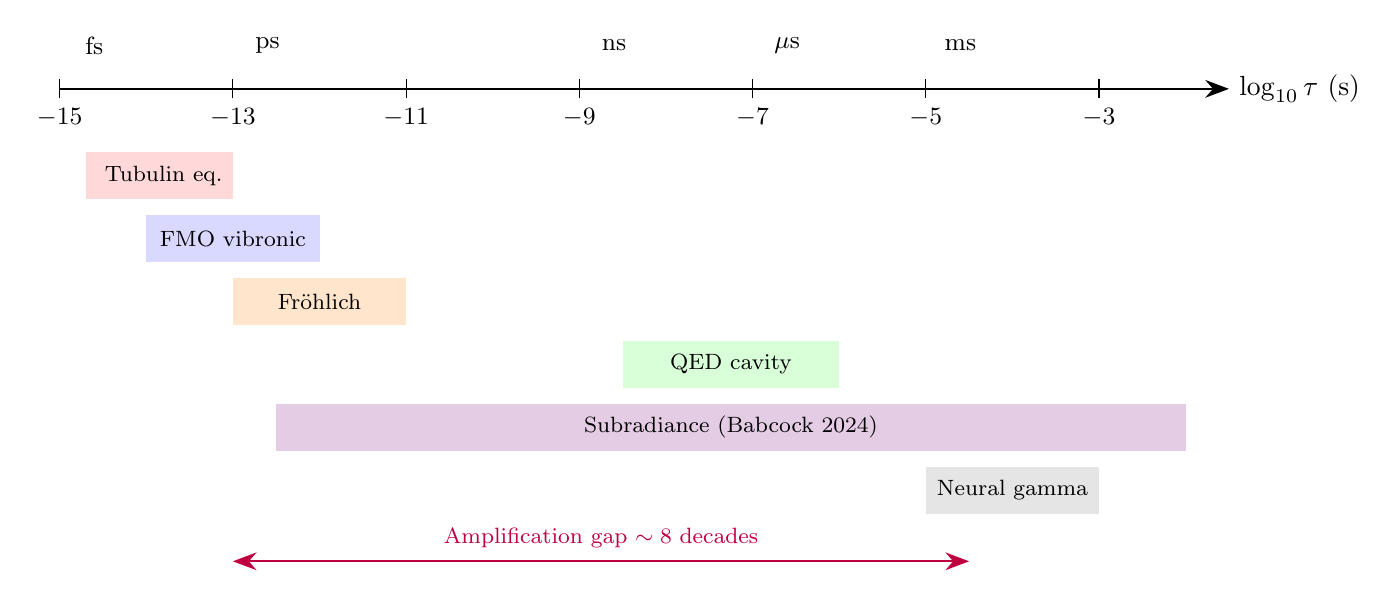
\begin{tikzpicture}[x=1.1cm,y=1cm,>={Stealth[length=3mm]}]
  % axis
  \draw[->,thick] (0,0) -- (13.5,0) node[right] {$\log_{10}\tau$~(s)};
  \foreach \x/\lab in {0/-15,2/-13,4/-11,6/-9,8/-7,10/-5,12/-3}{
    \draw (\x,0.12)--(\x,-0.12) node[below] {\small $\lab$};
  }
  \node at (0.4,0.55) {\small fs};
  \node at (2.4,0.55) {\small ps};
  \node at (6.4,0.55) {\small ns};
  \node at (8.4,0.55) {\small $\mu$s};
  \node at (10.4,0.55) {\small ms};
  % bands
  \fill[blue!15] (1.0,-2.2) rectangle (3.0,-1.6);
  \node[font=\footnotesize] at (2.0,-1.9) {FMO vibronic};
  \fill[red!15] (0.3,-1.4) rectangle (2.0,-0.8);
  \node[font=\footnotesize] at (1.2,-1.1) {Tubulin eq.};
  \fill[orange!20] (2.0,-3.0) rectangle (4.0,-2.4);
  \node[font=\footnotesize] at (3.0,-2.7) {Fr\"ohlich};
  \fill[green!15] (6.5,-3.8) rectangle (9.0,-3.2);
  \node[font=\footnotesize] at (7.75,-3.5) {QED cavity};
  \fill[violet!20] (2.5,-4.6) rectangle (13.0,-4.0);
  \node[font=\footnotesize] at (7.75,-4.3) {Subradiance (Babcock 2024)};
  \fill[gray!20] (10.0,-5.4) rectangle (12.0,-4.8);
  \node[font=\footnotesize] at (11.0,-5.1) {Neural gamma};
  % amplification arrow
  \draw[<->,thick,purple] (2.0,-6.0) -- (10.5,-6.0);
  \node[purple,font=\footnotesize] at (6.25,-5.7)
    {Amplification gap $\sim 8$~decades};
\end{tikzpicture}
\caption{Synthesis timeline. Equilibrium tubulin coherence (red) overlaps
the ultrafast molecular window and lies roughly 12 decades below neural gamma (grey).
Fr\"ohlich, QED-cavity, and subradiant channels are the candidate
bridges; only subradiance is already experimentally documented.}
\label{fig:timeline}
\end{figure*}



\section{Conclusions}

We have presented a comprehensive analysis of quantum coherence mechanisms
in microtubules with four main contributions: a calibrated open-system
baseline for equilibrium decoherence, an
FDT-rigorous quantum coherence utility framework (\S 3.4, including
quantum-discord refinement and comparison with Giovannetti-2004 /
Chin-2013), a perturbative scaling analysis of collective damping that
renders Fr\"ohlich condensation length-gated (\S 4.1.2), and the
integration of geometric subradiance as a third non-equilibrium channel
(\S\ref{sec:subradiance}), together with a Holstein vibronic analogue that
formalises the FMO--tubulin analogy (\S\ref{sec:holstein}).

\textbf{Equilibrium:} Vibrational dephasing limits coherence to
$T_2^* \approx 39\fs$ in the calibrated Ohmic release at 310~K. Even the
equilibrium upper bound remains sub-ps, and no cooperative equilibrium mechanism
circumvents this bound.

\textbf{Non-equilibrium:} Fr\"ohlich condensation potentially extends
coherence to $\tau \sim 10\text{--}100\ps$ but only for MTs longer than
$\sim 10\,\mu$m. QED cavity models predict $\tau \sim 0.1\text{--}1~\mu$s.
Geometric subradiance, already observed in related tryptophan mega-networks
\cite{Babcock2024}, reaches $\tau$ up to 10~s. These remain theoretical
proposals or preliminary observations; the discrepancy with Reimers et
al.\ \cite{Reimers2009} defines a central open question that we have now
rendered empirically resolvable.

\textbf{Classical sufficiency:} ING networks, gap junctions, ephaptic
coupling, and CTC quantitatively explain all observed neural
synchronization (\S 5.4). Information-theoretic analysis confirms no rate
advantage for quantum coherence under equilibrium assumptions (\S 5.5).

\textbf{Experimental priorities:} (1) Cavity spectroscopy---second-derivative
UV or THz---for direct test of QED cavity model, with ROC-based design
specifying SNR $\gtrsim 10^3$ as a conservative target and idealized BIC
crossing already in the few-$10^2$ range; (2) temperature-dependent 2D-IR
with cross/diagonal amplitude ratio of $\sim 3\text{--}5\%$ as
quantitative target; (3) kinetic isotope effects for tunneling;
(4) tau-knockdown-controlled MT disruption with synchronization precision
measurements; (5) length-resolved THz linewidth as direct
$\beta$-falsification test for Fr\"ohlich.

The amplification gap from picoseconds to milliseconds remains a hard
constraint, not a rhetorical one. Our utility framework sharpens that
constraint quantitatively and converts it into a testable experimental
agenda. In that sense, the contribution of this manuscript is twofold:
it narrows the plausible mechanism space under explicit assumptions, and
it specifies concrete falsification routes for cavity, Fr\"ohlich, and
subradiant scenarios without relying on overextended interpretative claims.


\section*{Ethics and Conflict of Interest}
The authors declare no financial or personal conflicts of interest. This work does not involve human or animal experimentation.

\section*{Acknowledgments}
We thank collaborators and colleagues for technical discussions on open quantum systems, HEOM benchmarking, and reproducibility workflows. Numerical analysis and visualization were performed with the Python scientific stack (NumPy, SciPy, Pandas, Matplotlib).

\section*{Author Contributions}
\textbf{Facundo Firmenich} led conceptualization, theoretical development, Bayesian convergence analysis, manuscript writing, and project coordination. \textbf{Pau Firmenich} contributed to computational pipeline design, reproducibility infrastructure, and validation workflows. \textbf{Le\'on Firmenich} contributed to methodological review, quality assurance, and editorial consolidation. All authors reviewed and approved the final manuscript.

\section*{AI-Assisted Development Disclosure}
This manuscript and associated codebase were developed with AI-assisted tooling for drafting support, refactoring assistance, consistency checks, and reproducibility orchestration. All scientific claims, equations, numerical interpretations, and final editorial decisions were validated and approved by the human authors.

\section*{Hardware Disclosure}
The reproducible computational workflow was designed to run on commodity hardware (including mid-range laptops) and does not require exclusive high-end HPC access for baseline reproduction. Runtime can vary by platform, but the deterministic workflow and documented outputs remain reproducible.

\section*{Data and code availability}
Code and reproducibility scripts are provided in the project repository under \texttt{git\_repo/}, including manuscript-oriented entrypoints and validation scripts for HEOM/Redfield and Bayesian convergence analysis.

For the small-$N$ HEOM convergence ledger, the current release includes a corrected Bayesian contraction layer (v2):
\texttt{src/bayesian\_heom\_hierarchy\_v2.py} with canonical input
\texttt{src/heom\_bayes\_input\_current.csv} and output folder
\texttt{heom\_bayes\_out\_v2/}. This layer infers contraction ratios on the
log scale with random-effects shrinkage, and is intended as a
Methods/Supplementary validation summary of existing convergence evidence.
It is not used as a substitute for new full-system HEOM production runs.

Repository: \url{https://github.com/biofisicaquantiqa/qmc_mt}

Canonical reproduction command (current release candidate): \texttt{python git\_repo/reproduce\_paper\_results.py}

Zenodo DOI: pending archival release (will be added in the camera-ready metadata pass).

\section{Figure placeholders for all generated artefacts}
\label{sec:all_figures_placeholders}

\begin{figure*}[t]
\centering
\begin{subfigure}[b]{0.48\textwidth}
\centering
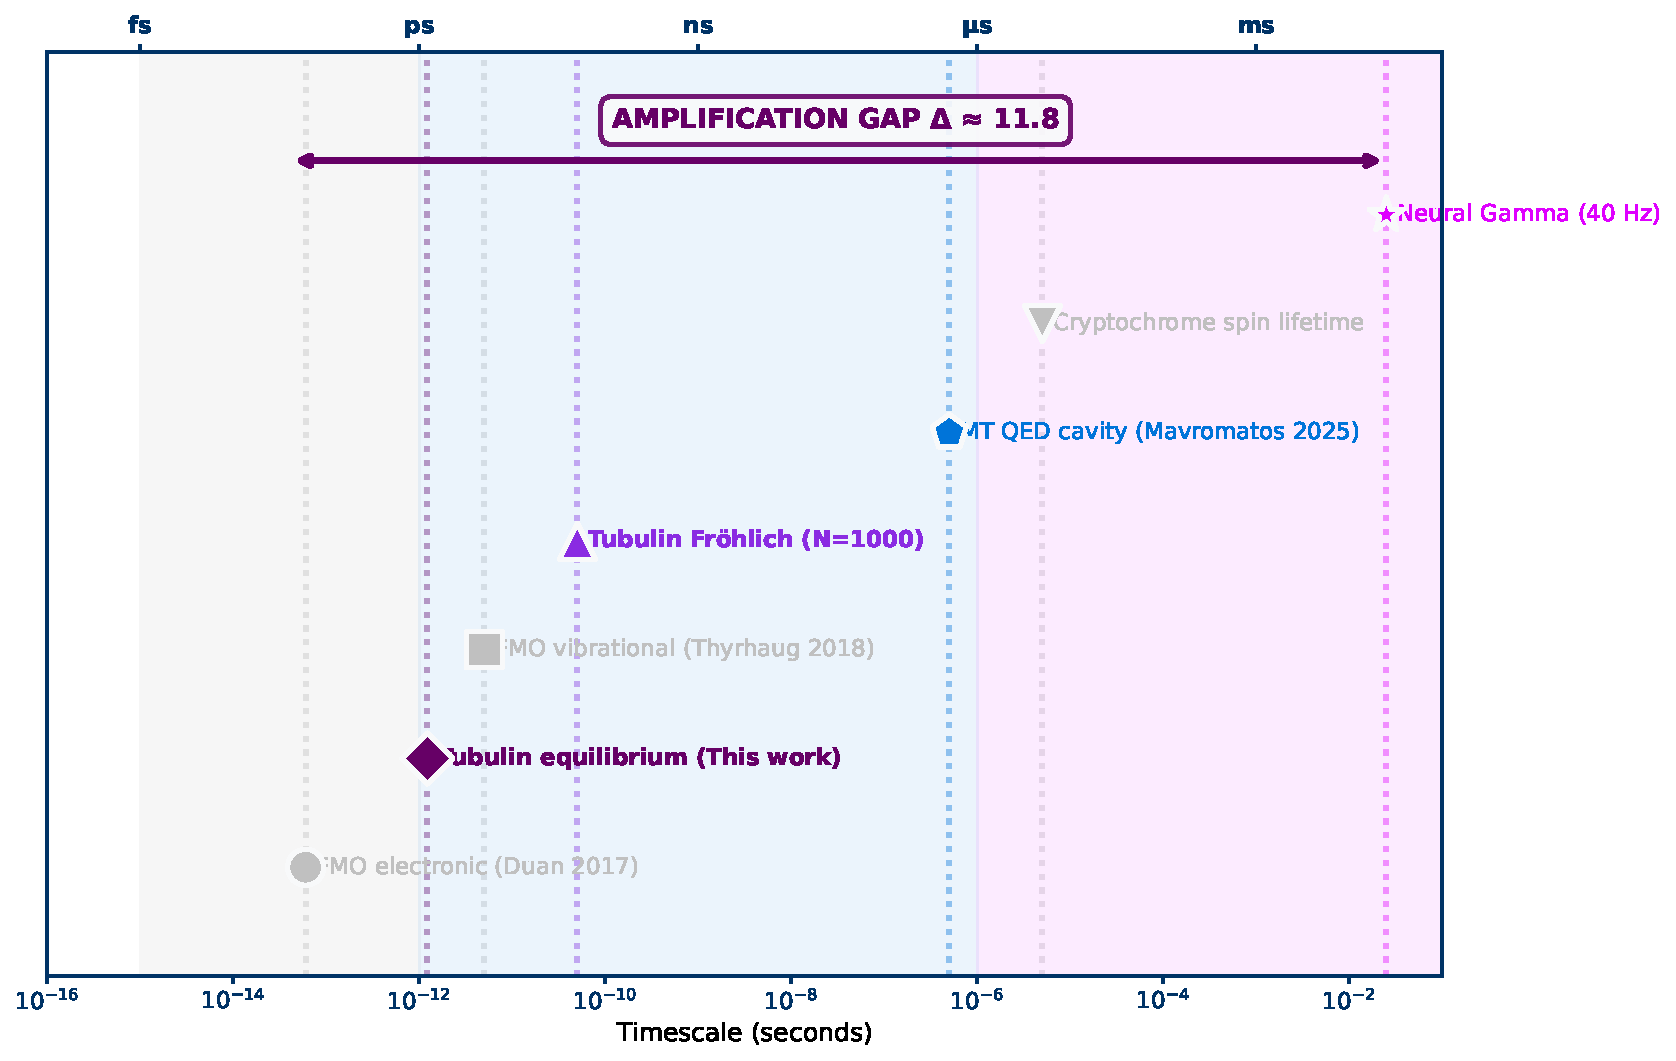
\includegraphics[width=\linewidth]{../figures_final/fig1_landscape.pdf}
\caption{Global timescale landscape.}
\end{subfigure}
\hfill
\begin{subfigure}[b]{0.48\textwidth}
\centering
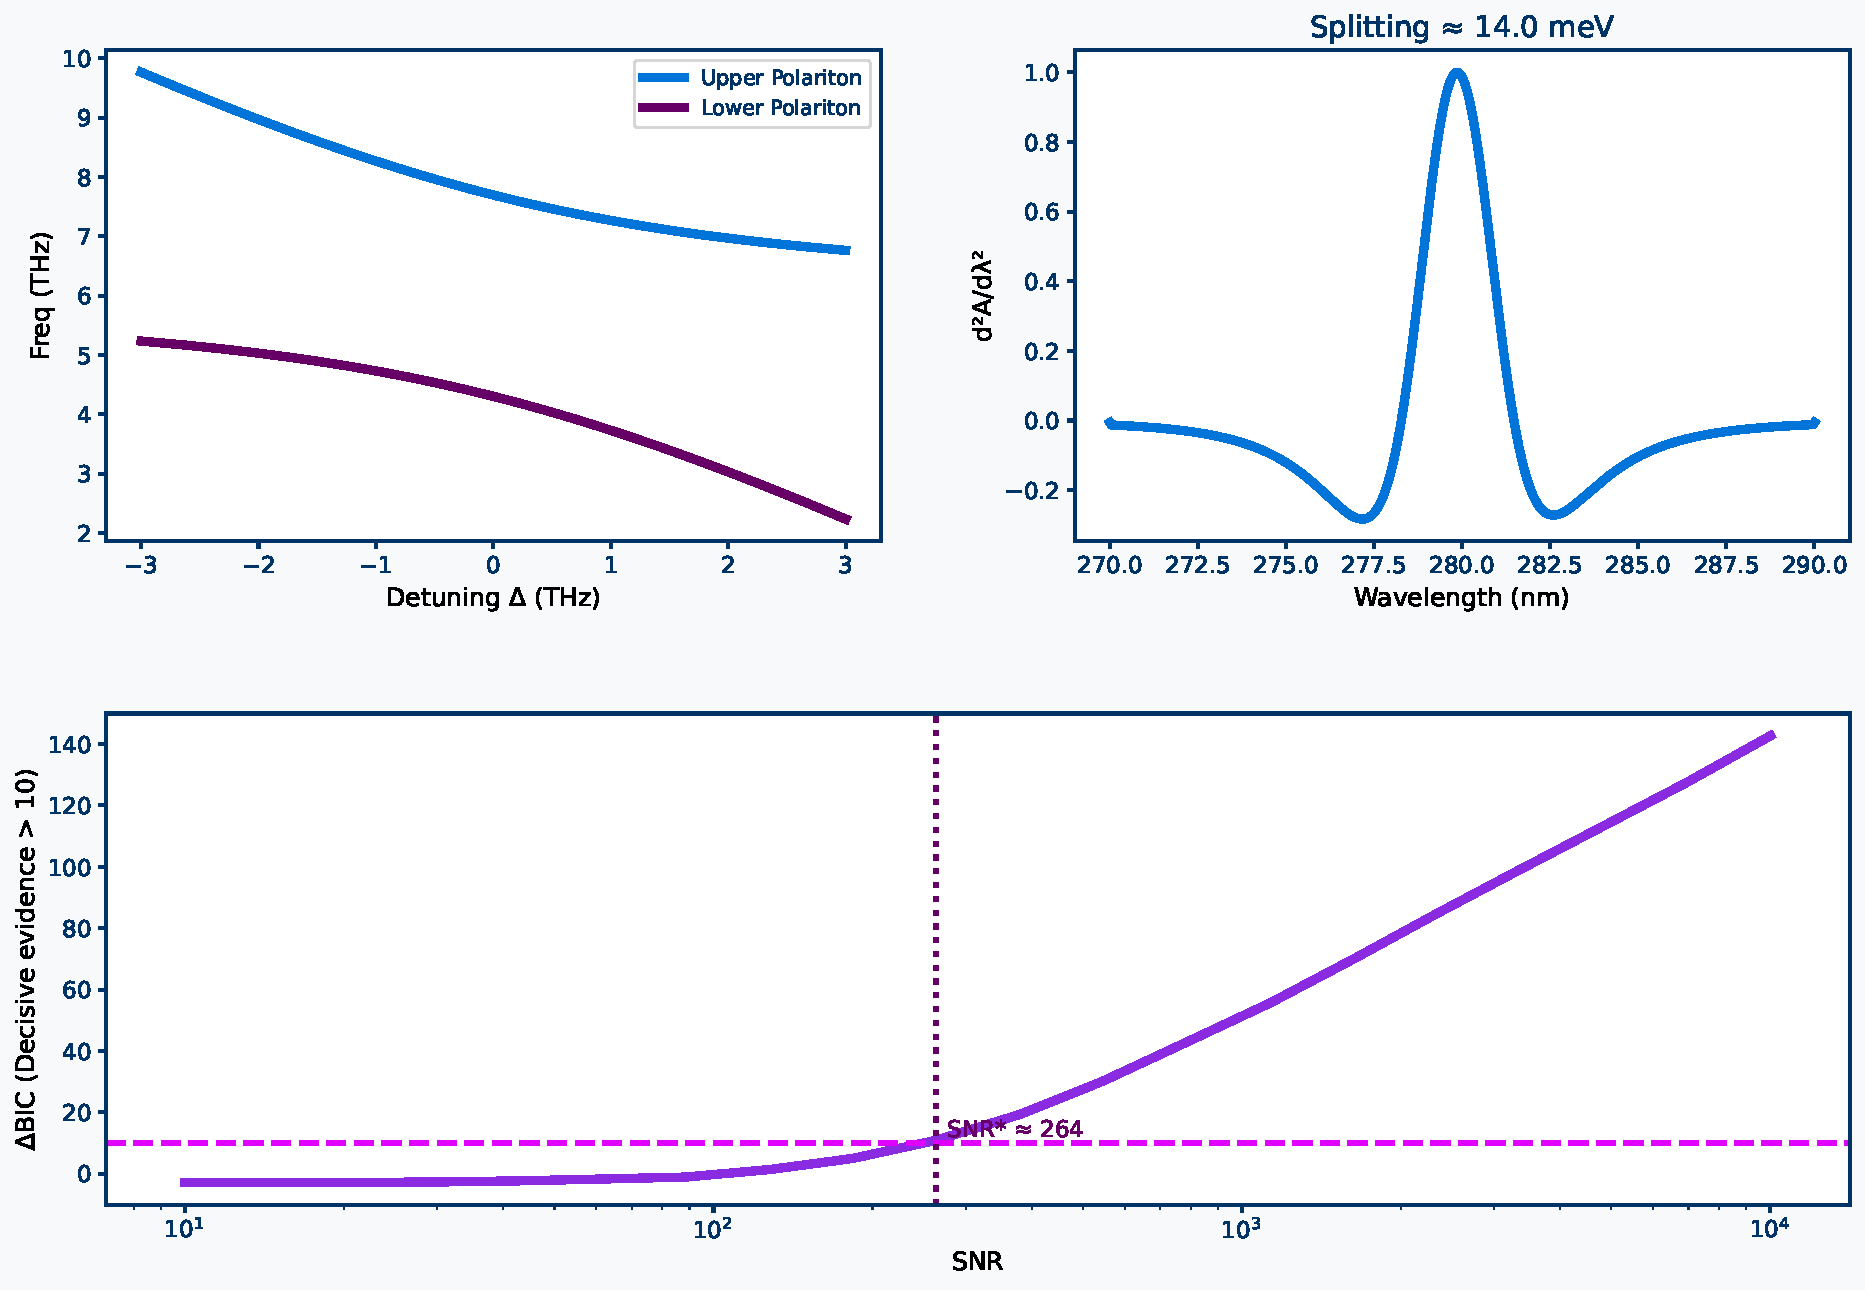
\includegraphics[width=\linewidth]{../figures_final/fig2_signatures.pdf}
\caption{Core signatures.}
\end{subfigure}
\caption{Primary figure placeholders I.}
\label{fig:paper_primary_i}
\end{figure*}

\begin{figure*}[t]
\centering
\begin{subfigure}[b]{0.48\textwidth}
\centering
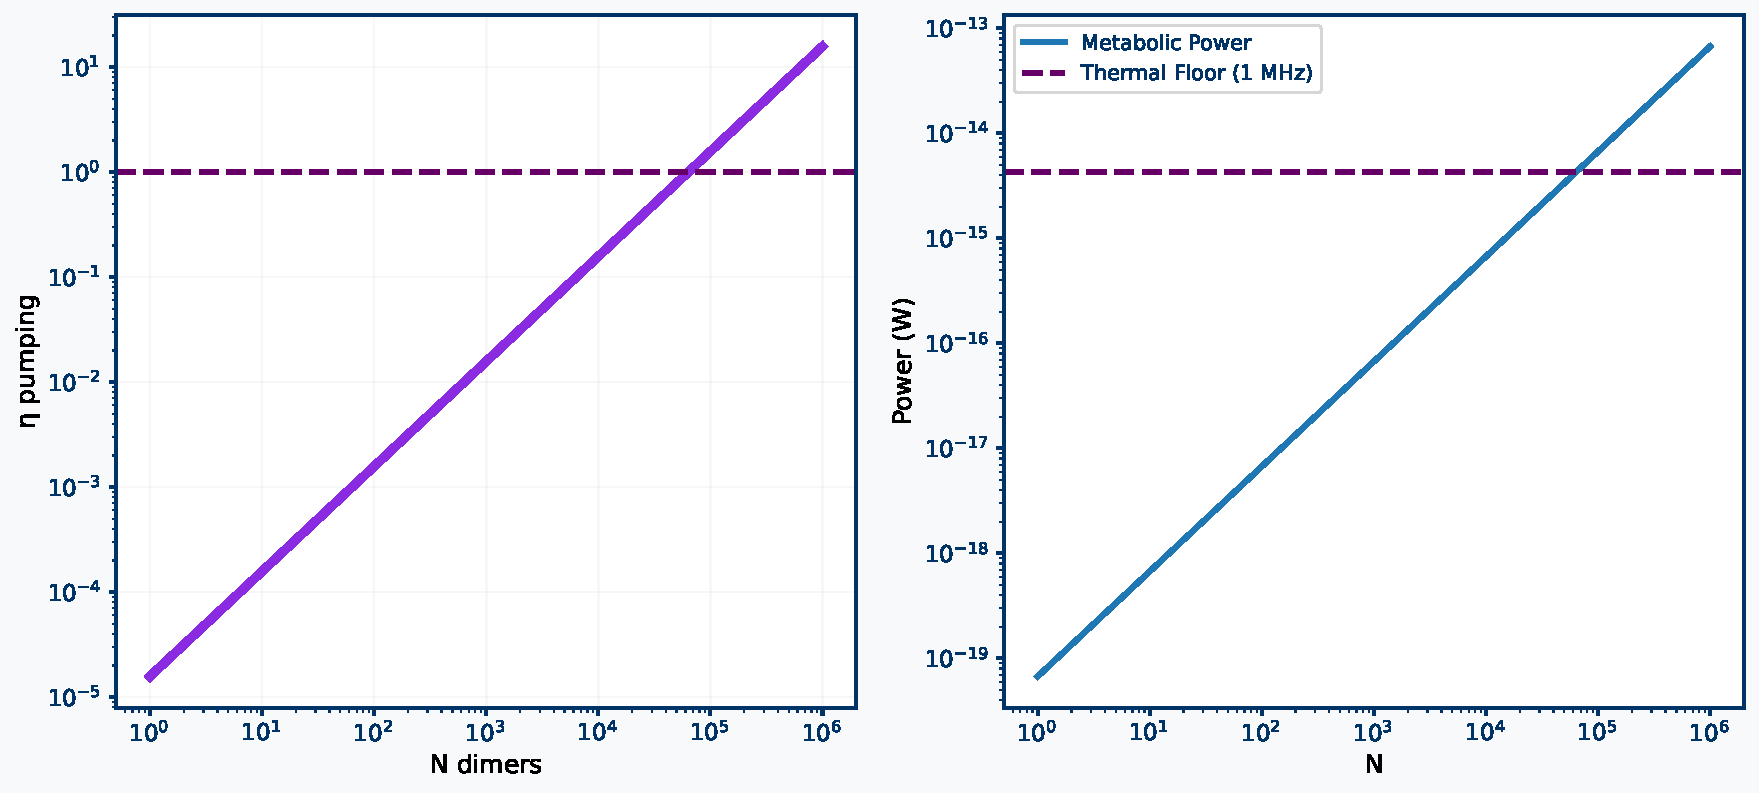
\includegraphics[width=\linewidth]{../figures_final/fig3_frohlich.pdf}
\caption{Fröhlich-related scaling.}
\end{subfigure}
\hfill
\begin{subfigure}[b]{0.48\textwidth}
\centering
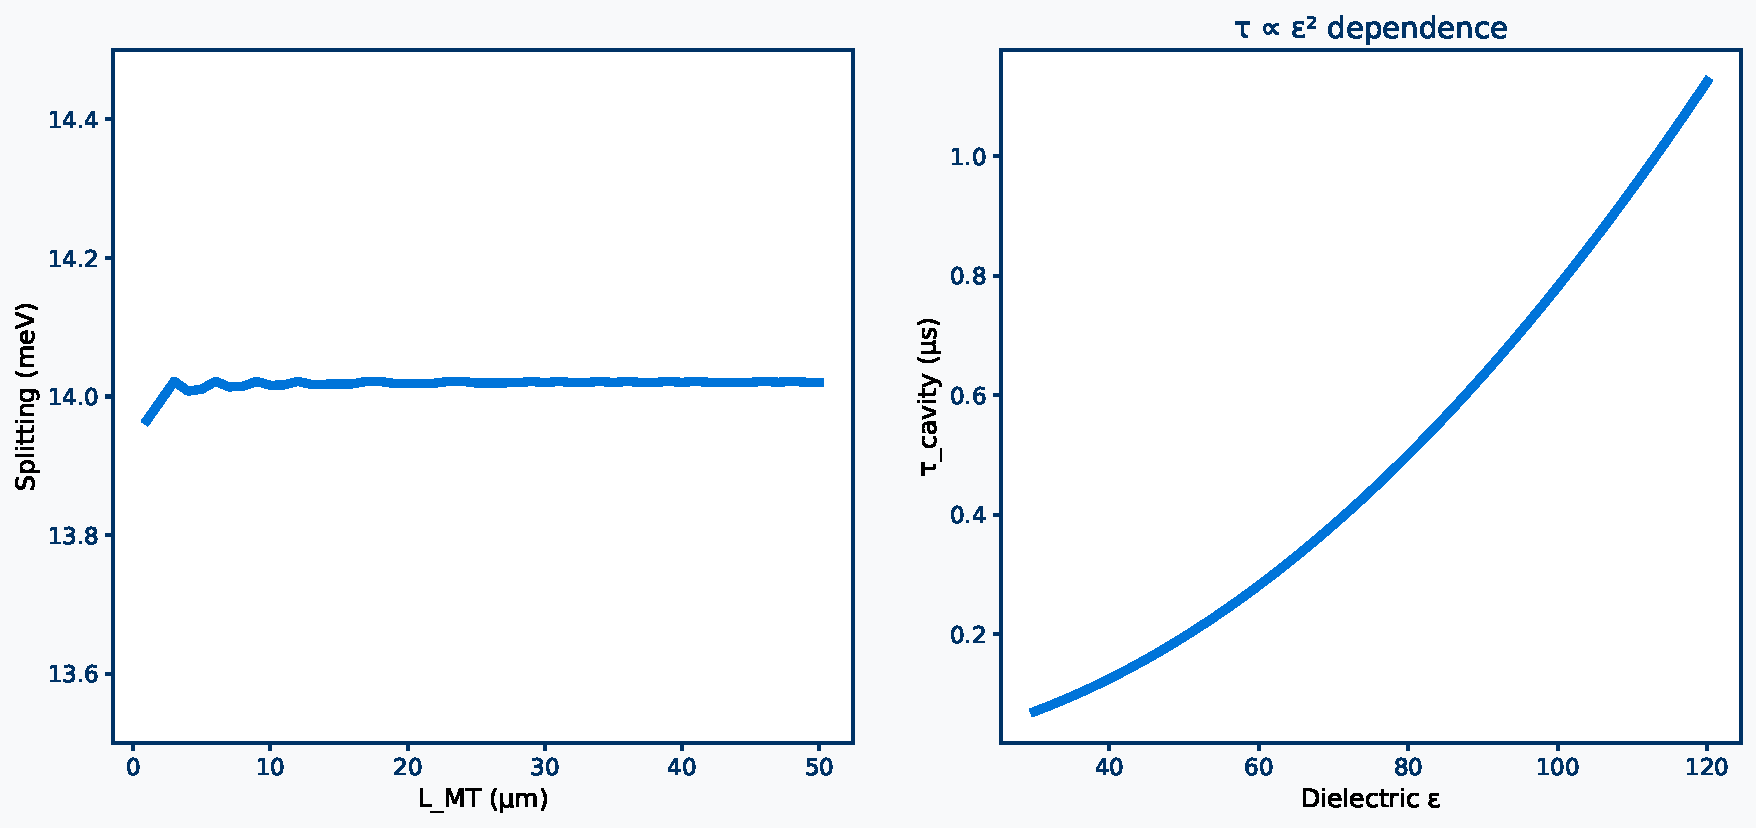
\includegraphics[width=\linewidth]{../figures_final/fig4_scaling.pdf}
\caption{System-level scaling.}
\end{subfigure}
\caption{Primary figure placeholders II.}
\label{fig:paper_primary_ii}
\end{figure*}

\begin{figure*}[t]
\centering
\begin{subfigure}[b]{0.48\textwidth}
\centering
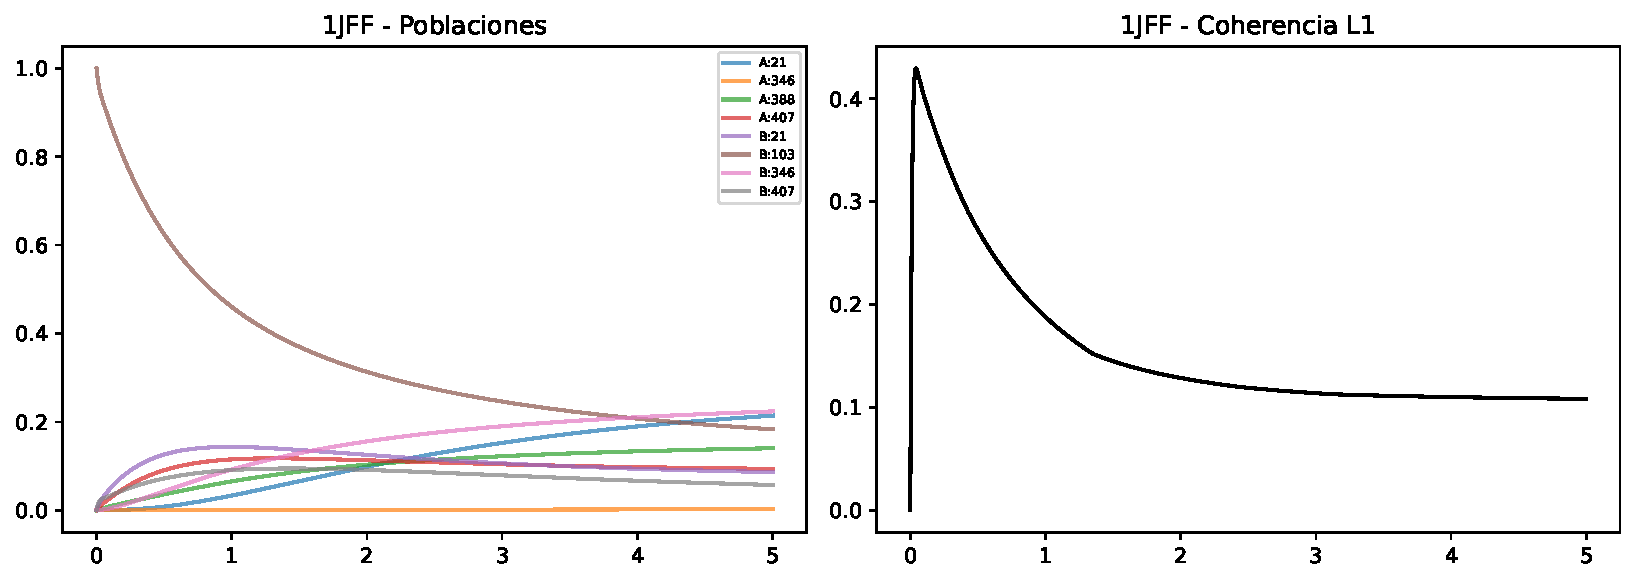
\includegraphics[width=\linewidth]{../figures_final/redfield_1JFF.pdf}
\caption{Redfield 1JFF.}
\end{subfigure}
\hfill
\begin{subfigure}[b]{0.48\textwidth}
\centering
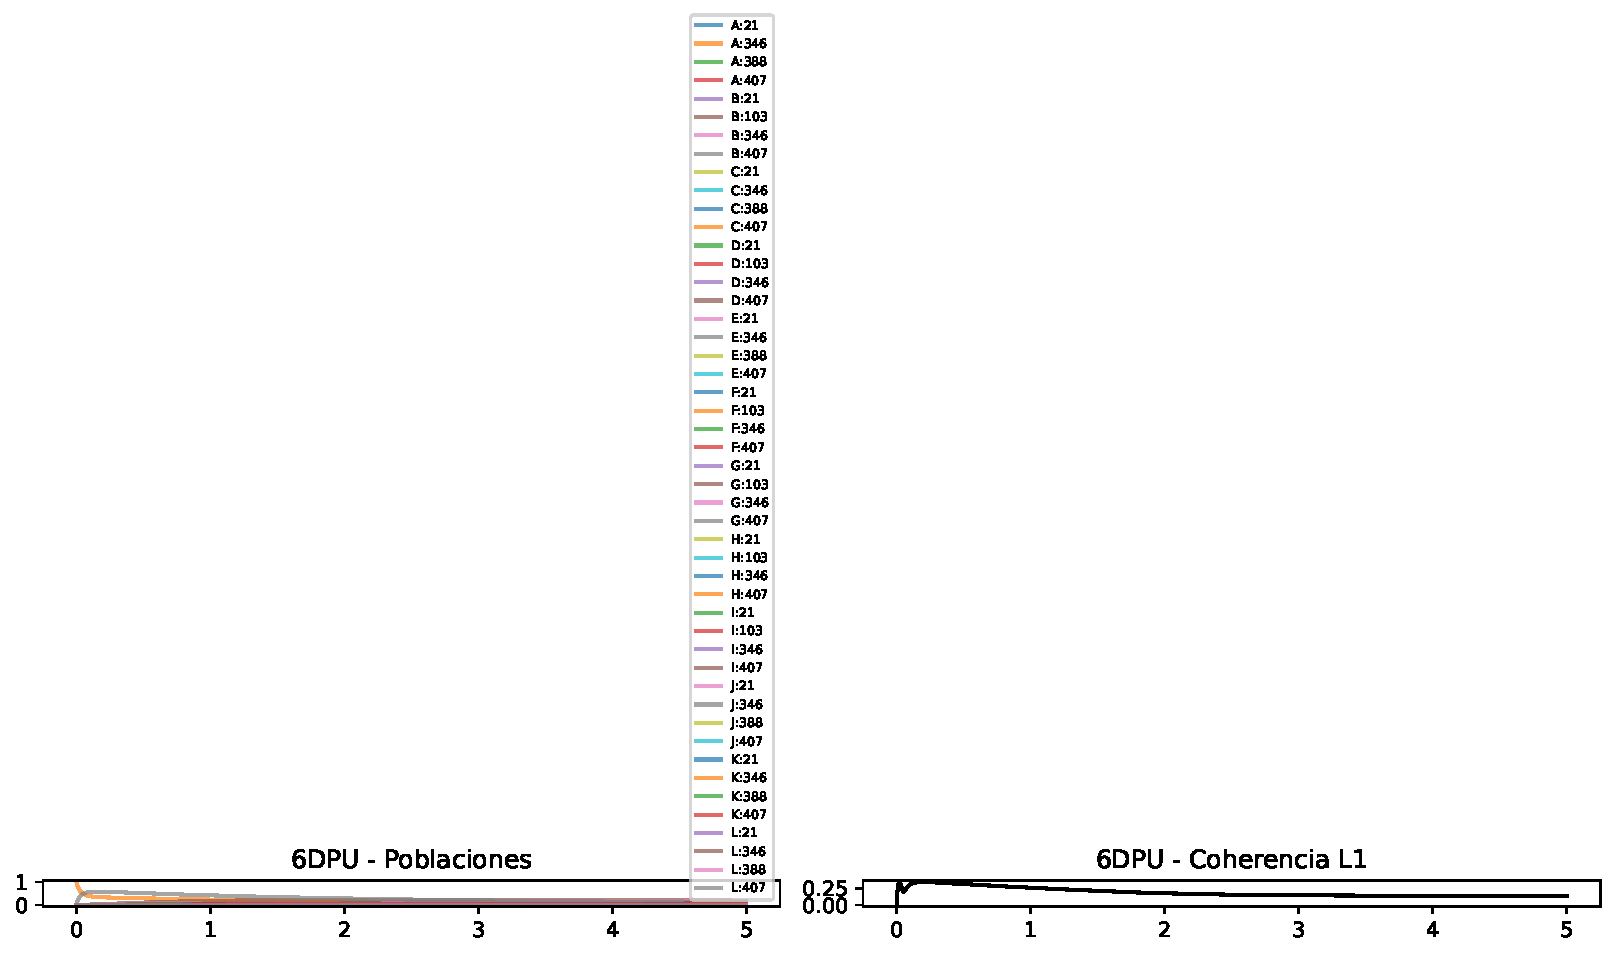
\includegraphics[width=\linewidth]{../figures_final/redfield_6DPU.pdf}
\caption{Redfield 6DPU.}
\end{subfigure}
\caption{Additional model placeholders.}
\label{fig:paper_additional_models}
\end{figure*}

\appendix

\section{Methodological appendices}
\label{app:methodological}

\begin{figure*}[t]
\centering
\begin{subfigure}[b]{0.48\textwidth}
\centering
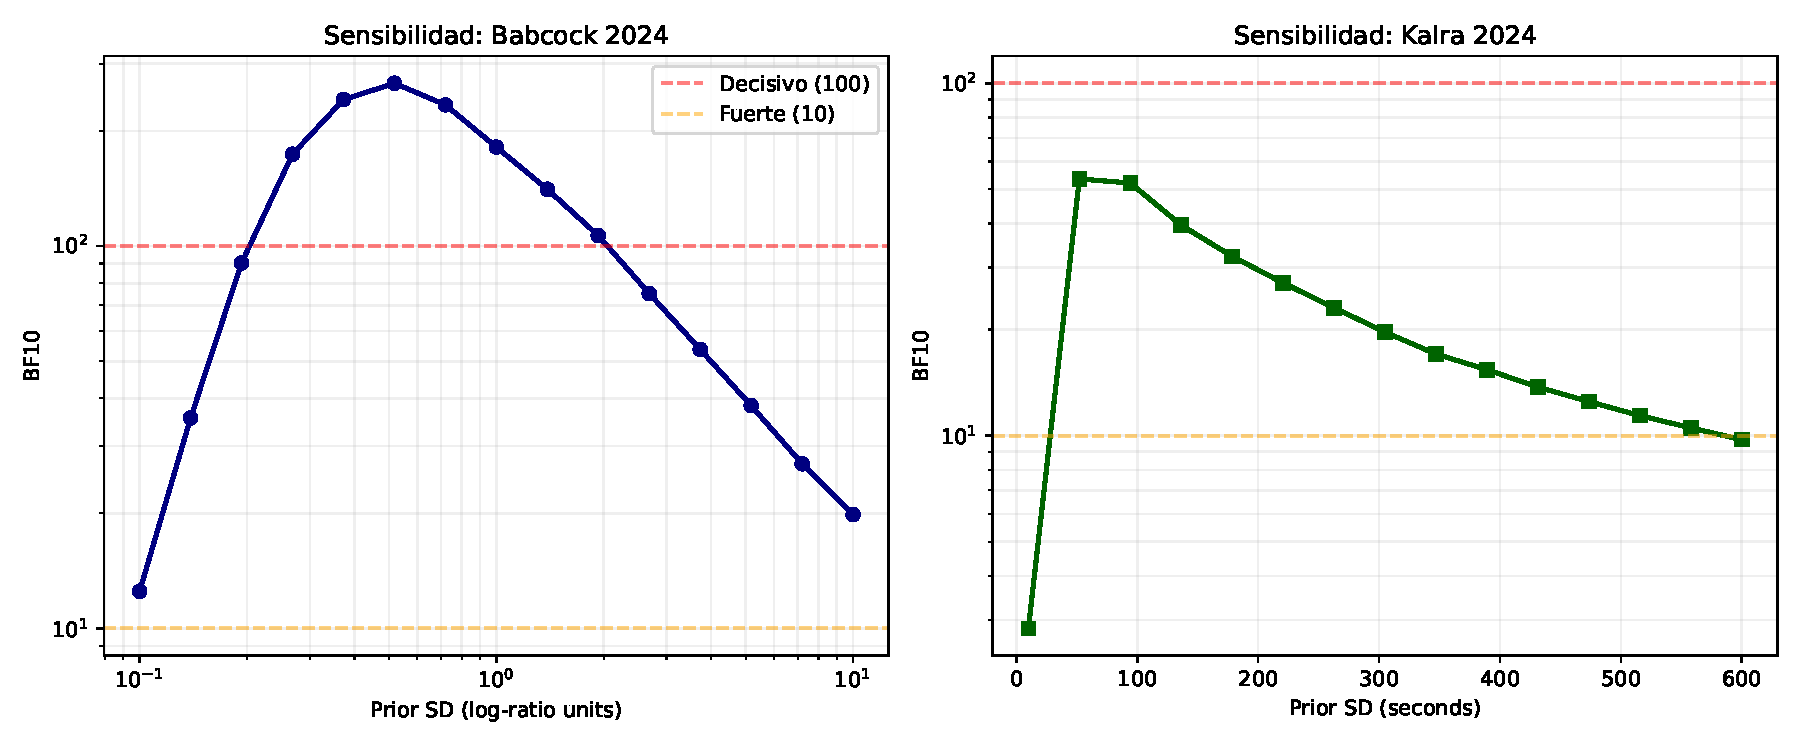
\includegraphics[width=\linewidth]{../figures_final/prior_sensitivity.pdf}
\caption{Prior sensitivity.}
\end{subfigure}
\hfill
\begin{subfigure}[b]{0.48\textwidth}
\centering
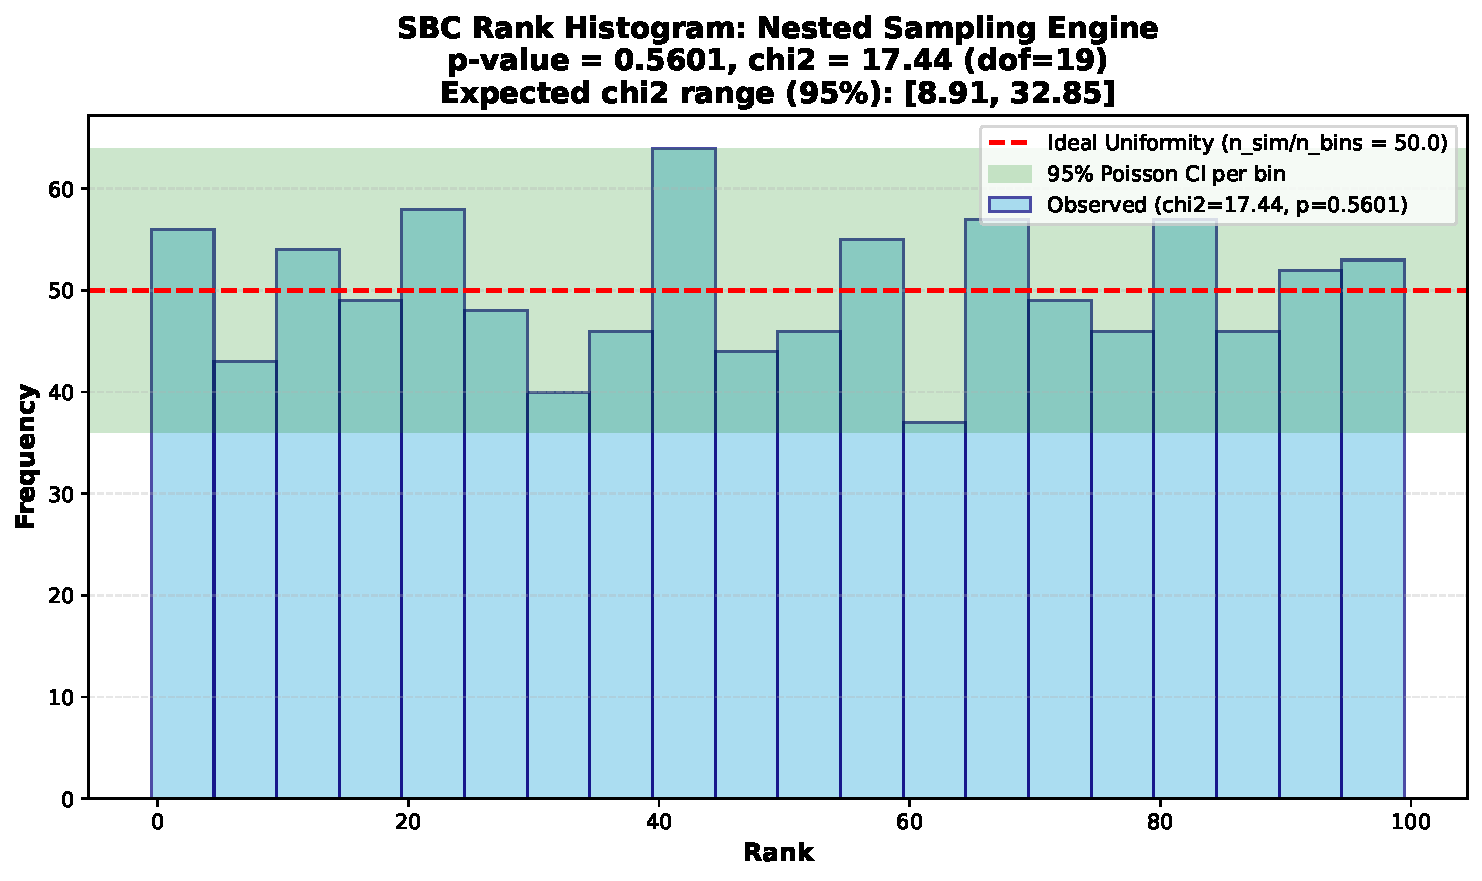
\includegraphics[width=\linewidth]{../figures_final/sbc_calibration_ns.pdf}
\caption{SBC calibration.}
\end{subfigure}
\caption{Methodological and calibration diagnostics placeholders.}
\label{fig:app_method_diag}
\end{figure*}

\section{Statistical appendices}
\label{app:statistical}

\begin{figure*}[t]
\centering
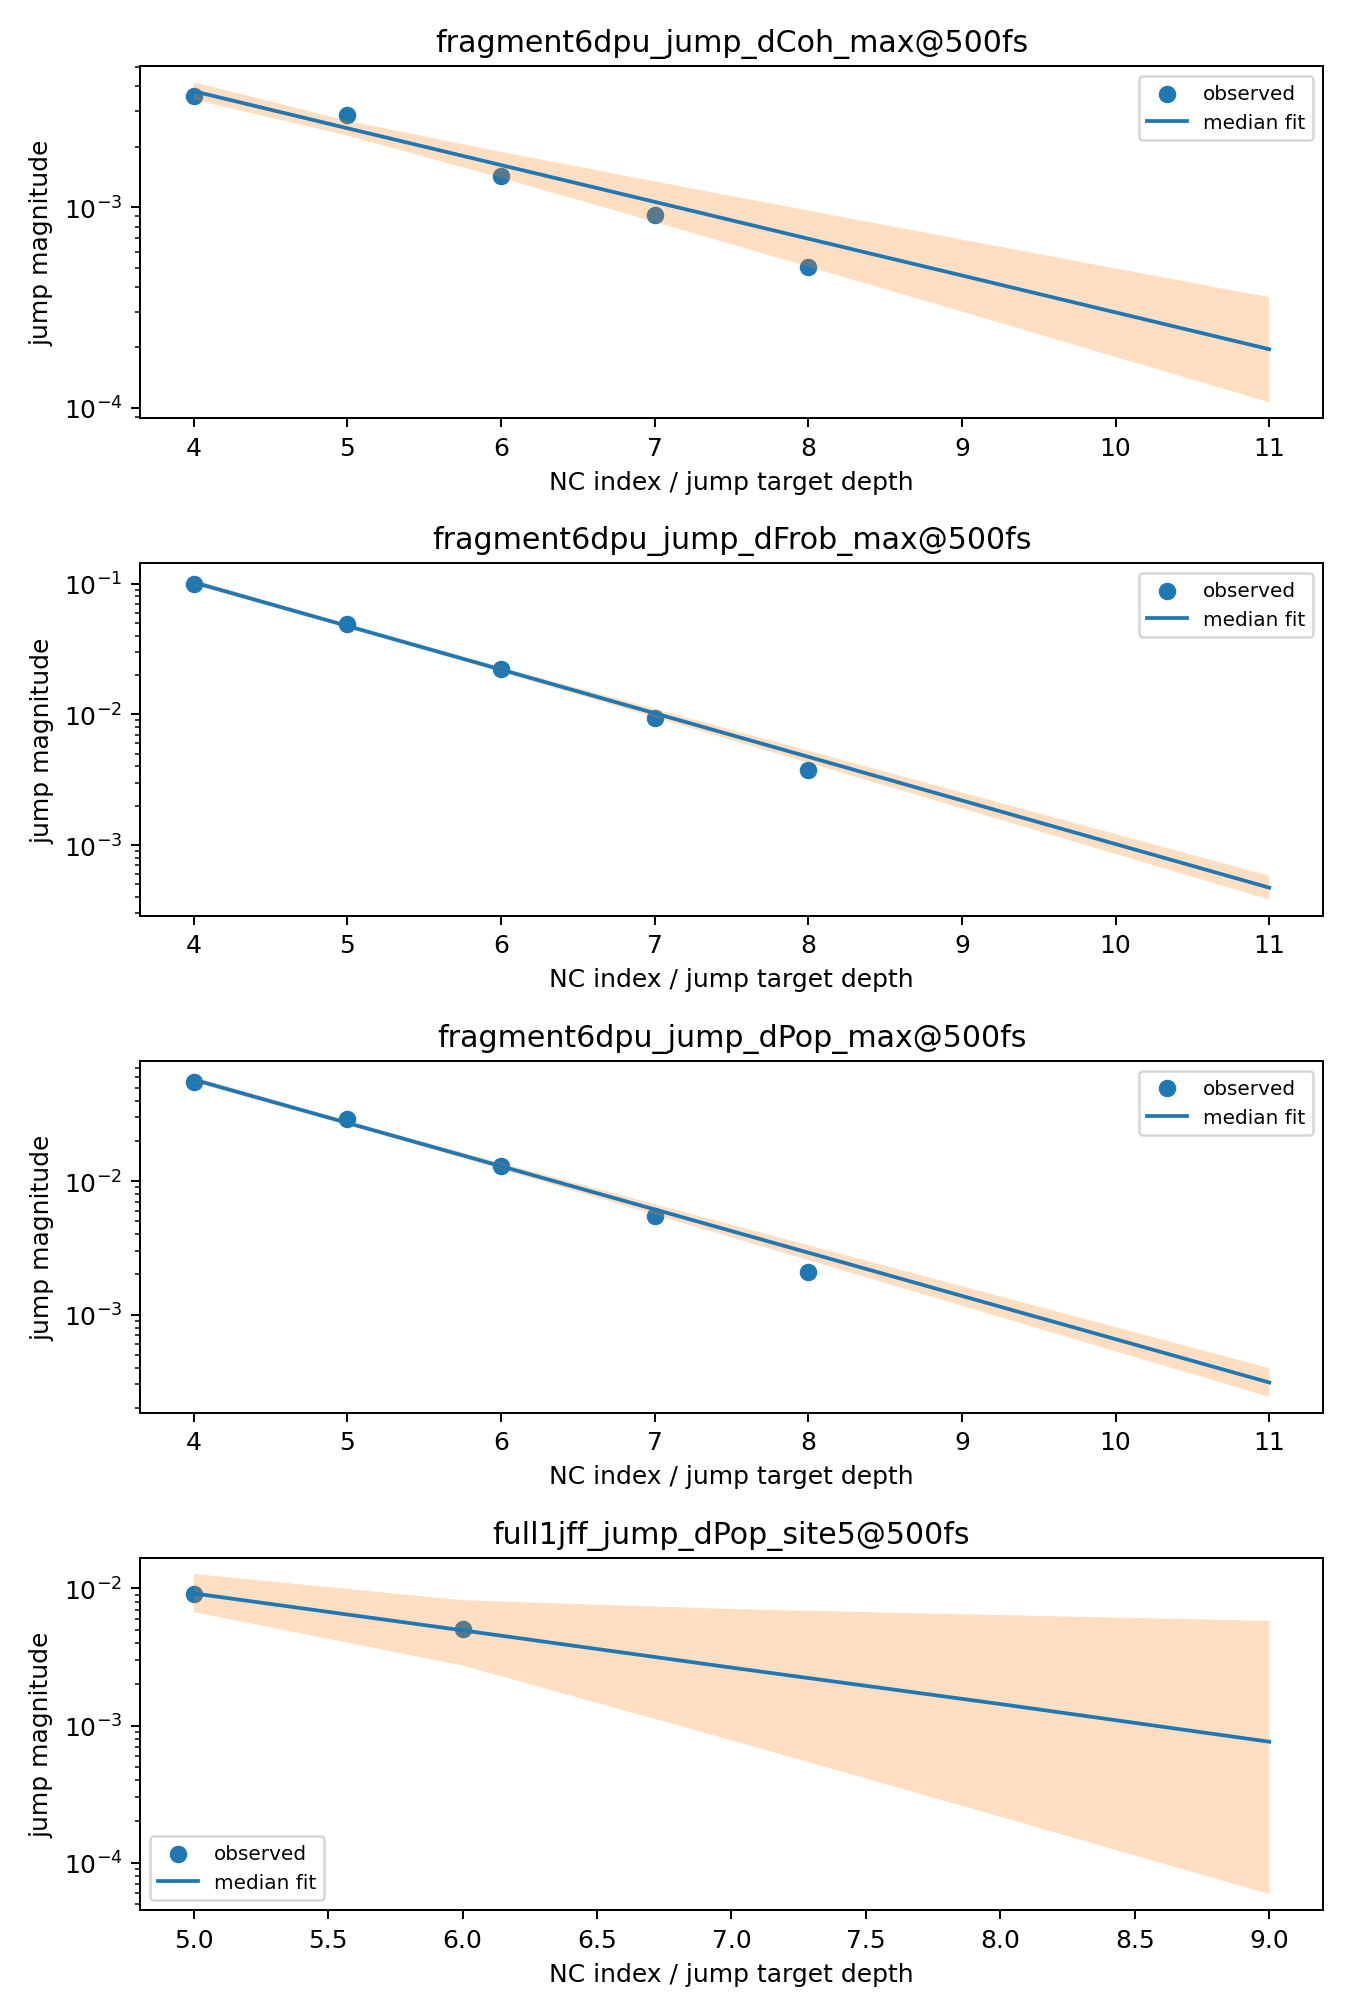
\includegraphics[width=0.75\textwidth]{../heom_bayes_out_v2/posterior_plots_v2.png}
\caption{Bayesian hierarchy posterior diagnostics placeholder.}
\label{fig:app_bayes_diag}
\end{figure*}

\noindent\textbf{Companion statistical artefacts (tabular/JSON/CSV).}
The corresponding statistical outputs are available in repository artefacts
(e.g., \texttt{sbc\_report.json}, \texttt{prior\_sensitivity.json},
\texttt{validation\_report.json}, and
\texttt{heom\_bayes\_out\_v2/*.csv}) and complement the figure placeholders above.

\begin{thebibliography}{99}

\bibitem{Engel2007} G.~S.~Engel \textit{et al.}, \textit{Nature}
\textbf{446}, 782 (2007).
\bibitem{Panitchayangkoon2010} G.~Panitchayangkoon \textit{et al.},
\textit{Proc.\ Natl.\ Acad.\ Sci.\ USA} \textbf{107}, 12766 (2010).
\bibitem{Duan2017} H.-G.~Duan \textit{et al.},
\textit{Proc.\ Natl.\ Acad.\ Sci.\ USA} \textbf{114}, 8493 (2017).
\bibitem{Thyrhaug2018} E.~Thyrhaug \textit{et al.},
\textit{Nat.\ Chem.} \textbf{10}, 780 (2018).
\bibitem{Thyrhaug2022b} E.~Thyrhaug \textit{et al.},
\textit{J.\ Phys.\ Chem.\ Lett.} \textbf{9}, 6412 (2018).
\bibitem{Tiwari2013} V.~Tiwari, W.~K.~Peters, and D.~M.~Jonas,
\textit{Proc.\ Natl.\ Acad.\ Sci.\ USA} \textbf{110}, 1203 (2013).
\bibitem{Christensson2012} N.~Christensson \textit{et al.},
\textit{J.\ Phys.\ Chem.\ B} \textbf{116}, 7449 (2012).
\bibitem{Tempelaar2014} R.~Tempelaar, T.~L.~C.~Jansen, and J.~Knoester,
\textit{J.\ Phys.\ Chem.\ B} \textbf{118}, 12865 (2014).
\bibitem{Dean2017} J.~C.~Dean and G.~D.~Scholes,
\textit{Acc.\ Chem.\ Res.} \textbf{50}, 2746 (2017).
\bibitem{Plenio2008} M.~B.~Plenio and S.~F.~Huelga,
\textit{New J.\ Phys.} \textbf{10}, 113019 (2008).
\bibitem{Cao2020} J.~Cao \textit{et al.},
\textit{Sci.\ Adv.} \textbf{6}, eaaz4888 (2020).
\bibitem{Chin2013} A.~W.~Chin, J.~Prior, R.~Rosenbach, F.~Caycedo-Soler,
S.~F.~Huelga, and M.~B.~Plenio,
\textit{Nat.\ Phys.} \textbf{9}, 113 (2013).
\bibitem{Ritz2000} T.~Ritz, S.~Adem, and K.~Schulten,
\textit{Biophys.\ J.} \textbf{78}, 707 (2000).
\bibitem{Maeda2012} K.~Maeda \textit{et al.},
\textit{Proc.\ Natl.\ Acad.\ Sci.\ USA} \textbf{109}, 4774 (2012).
\bibitem{Gauger2011} E.~M.~Gauger \textit{et al.},
\textit{Phys.\ Rev.\ Lett.} \textbf{106}, 040503 (2011).
\bibitem{Scrutton1999} N.~S.~Scrutton, J.~Basran, and M.~J.~Sutcliffe,
\textit{Eur.\ J.\ Biochem.} \textbf{264}, 666 (1999).
\bibitem{Klinman2013} J.~P.~Klinman and A.~Kohen,
\textit{Annu.\ Rev.\ Biochem.} \textbf{82}, 471 (2013).
\bibitem{Babcock2024} N.~S.~Babcock \textit{et al.},
\textit{J.\ Phys.\ Chem.\ B} \textbf{128}, 4035 (2024).
\bibitem{Celardo2019} G.~L.~Celardo, A.~Ferretti, and R.~Kaiser,
\textit{New J.\ Phys.} \textbf{21}, 023012 (2019).
\bibitem{Dicke1954} R.~H.~Dicke,
\textit{Phys.\ Rev.} \textbf{93}, 99 (1954).
\bibitem{Gross1982} M.~Gross and S.~Haroche,
\textit{Phys.\ Rep.} \textbf{93}, 301 (1982).
\bibitem{Mavromatos2025} N.~E.~Mavromatos, A.~Mershin, and D.~V.~Nanopoulos,
\textit{Eur.\ Phys.\ J.\ Plus} \textbf{140}, 1116 (2025).
\bibitem{Mavromatos1997} N.~E.~Mavromatos and D.~V.~Nanopoulos,
\textit{Int.\ J.\ Mod.\ Phys.\ B} \textbf{11}, 851 (1997).
\bibitem{Mavromatos2002} N.~E.~Mavromatos, A.~Mershin, and D.~V.~Nanopoulos,
\textit{Int.\ J.\ Mod.\ Phys.\ B} \textbf{16}, 3623 (2002).
\bibitem{DelGiudice1988} E.~Del~Giudice, G.~Preparata, and G.~Vitiello,
\textit{Phys.\ Rev.\ Lett.} \textbf{61}, 1085 (1988).
\bibitem{Sahu2013} S.~Sahu \textit{et al.},
\textit{Biosens.\ Bioelectron.} \textbf{47}, 141 (2013).
\bibitem{Tuszynski1995} J.~A.~Tuszy\'nski \textit{et al.},
\textit{J.\ Theor.\ Biol.} \textbf{174}, 371 (1995).
\bibitem{Frohlich1968} H.~Fr\"ohlich,
\textit{Phys.\ Lett.\ A} \textbf{26}, 402 (1968).
\bibitem{Frohlich1977} H.~Fr\"ohlich,
\textit{Riv.\ Nuovo Cimento} \textbf{7}, 399 (1977).
\bibitem{Reimers2009} J.~R.~Reimers \textit{et al.},
\textit{Proc.\ Natl.\ Acad.\ Sci.\ USA} \textbf{106}, 4219 (2009).
\bibitem{Pokorn2011} J.~Pokorn\'y, J.~Ha\v{s}ek, and F.~Jel\'inek,
\textit{J.\ Phys.:\ Conf.\ Ser.} \textbf{329}, 012013 (2011).
\bibitem{Salari2011} V.~Salari \textit{et al.},
\textit{J.\ Phys.:\ Conf.\ Ser.} \textbf{306}, 012075 (2011).
\bibitem{Khan2024} S.~Khan \textit{et al.},
\textit{eNeuro} \textbf{11}, ENEURO.0532-23.2024 (2024).
\bibitem{Kalra2023} A.~P.~Kalra \textit{et al.},
\textit{ACS Cent.\ Sci.} \textbf{9}, 352 (2023).
\bibitem{Wiest2025} M.~C.~Wiest,
\textit{Neurosci.\ Conscious.} \textbf{2025}, niaf011 (2025).
\bibitem{Saxena2020} K.~Saxena \textit{et al.},
\textit{Fractal Fract.} \textbf{4}, 11 (2020).
\bibitem{Singh2021} P.~Singh \textit{et al.},
\textit{J.\ Neurophysiol.} \textbf{125}, 2107 (2021).
\bibitem{Tegmark2000} M.~Tegmark,
\textit{Phys.\ Rev.\ E} \textbf{61}, 4194 (2000).
\bibitem{Hagan2002} S.~Hagan, S.~R.~Hameroff, and J.~A.~Tuszy\'nski,
\textit{Phys.\ Rev.\ E} \textbf{65}, 061901 (2002).
\bibitem{May2011} V.~May and O.~K\"uhn, \textit{Charge and Energy Transfer
Dynamics in Molecular Systems}, 3rd ed.\ (Wiley-VCH, 2011).
\bibitem{Rego2003} L.~G.~C.~Rego \textit{et al.},
\textit{J.\ Am.\ Chem.\ Soc.} \textbf{125}, 7989 (2003).
\bibitem{Xiang2019} Z.~Xiang, C.~Tang, and L.~Xin,
\textit{Chin.\ Phys.\ B} \textbf{28}, 048701 (2019).
\bibitem{Eaves2005} J.~D.~Eaves \textit{et al.},
\textit{Proc.\ Natl.\ Acad.\ Sci.\ USA} \textbf{102}, 13019 (2005).
\bibitem{Israelachvili2011} J.~N.~Israelachvili, \textit{Intermolecular and
Surface Forces}, 3rd ed.\ (Academic Press, 2011).
\bibitem{Weiss2008} U.~Weiss, \textit{Quantum Dissipative Systems},
3rd ed.\ (World Scientific, 2008).
\bibitem{Kubo1966} R.~Kubo,
\textit{Rep.\ Prog.\ Phys.} \textbf{29}, 255 (1966).
\bibitem{BreuerPetruccione2002} H.-P.~Breuer and F.~Petruccione,
\textit{The Theory of Open Quantum Systems} (Oxford Univ.\ Press, 2002).
\bibitem{Ishizaki2009} A.~Ishizaki and G.~R.~Fleming,
\textit{J.\ Chem.\ Phys.} \textbf{130}, 234111 (2009).
\bibitem{Tanimura2020} Y.~Tanimura,
\textit{J.\ Chem.\ Phys.} \textbf{153}, 020901 (2020).
\bibitem{Nogales1998} E.~Nogales, S.~G.~Wolf, and K.~H.~Downing,
\textit{Nature} \textbf{391}, 199 (1998).
\bibitem{Adolphs2006} J.~Adolphs and T.~Renger,
\textit{Biophys.\ J.} \textbf{91}, 2778 (2006).
\bibitem{Sept2003} D.~Sept, N.~A.~Baker, and J.~A.~McCammon,
\textit{Protein Sci.} \textbf{12}, 2257 (2003).
\bibitem{Moix2017} J.~M.~Moix \textit{et al.},
\textit{J.\ Phys.\ Chem.\ B} \textbf{121}, 3024 (2017).
\bibitem{Zurek2003} W.~H.~Zurek,
\textit{Rev.\ Mod.\ Phys.} \textbf{75}, 715 (2003).
\bibitem{Holstein1959} T.~Holstein,
\textit{Ann.\ Phys.\ (NY)} \textbf{8}, 325 (1959).
\bibitem{Mukamel1995} S.~Mukamel, \textit{Principles of Nonlinear Optical
Spectroscopy} (Oxford Univ.\ Press, 1995).
\bibitem{Hamm2011} P.~Hamm and M.~Zanni, \textit{Concepts and Methods of
2D Infrared Spectroscopy} (Cambridge Univ.\ Press, 2011).
\bibitem{Ollivier2001} H.~Ollivier and W.~H.~Zurek,
\textit{Phys.\ Rev.\ Lett.} \textbf{88}, 017901 (2001).
\bibitem{Luo2008} S.~Luo,
\textit{Phys.\ Rev.\ A} \textbf{77}, 042303 (2008).
\bibitem{Knill1998} E.~Knill and R.~Laflamme,
\textit{Phys.\ Rev.\ Lett.} \textbf{81}, 5672 (1998).
\bibitem{Datta2008} A.~Datta, A.~Shaji, and C.~M.~Caves,
\textit{Phys.\ Rev.\ Lett.} \textbf{100}, 050502 (2008).
\bibitem{Borgers2003} C.~B\"orgers and N.~Kopell,
\textit{Neural Comput.} \textbf{15}, 509 (2003).
\bibitem{Brunel2003} N.~Brunel and X.-J.~Wang,
\textit{J.\ Neurophysiol.} \textbf{90}, 415 (2003).
\bibitem{Buzsaki2012} G.~Buzs\'aki and X.-J.~Wang,
\textit{Annu.\ Rev.\ Neurosci.} \textbf{35}, 203 (2012).
\bibitem{Fries2001} P.~Fries \textit{et al.},
\textit{Science} \textbf{291}, 1560 (2001).
\bibitem{Buschman2007} T.~J.~Buschman and E.~K.~Miller,
\textit{Science} \textbf{315}, 1860 (2007).
\bibitem{Cardin2009} J.~A.~Cardin \textit{et al.},
\textit{Nature} \textbf{459}, 663 (2009).
\bibitem{Fries2015} P.~Fries,
\textit{Neuron} \textbf{88}, 220 (2015).
\bibitem{Poirazi2020} P.~Poirazi and A.~Papoutsi,
\textit{Nat.\ Rev.\ Neurosci.} \textbf{21}, 303 (2020).
\bibitem{Galarreta1999} M.~Galarreta and S.~Hestrin,
\textit{Nature} \textbf{402}, 72 (1999).
\bibitem{Bennett2004} M.~V.~L.~Bennett and R.~S.~Zukin,
\textit{Neuron} \textbf{41}, 495 (2004).
\bibitem{Anastassiou2011} C.~A.~Anastassiou \textit{et al.},
\textit{Nat.\ Neurosci.} \textbf{14}, 217 (2011).
\bibitem{Frohlich2010} F.~Fr\"ohlich and D.~A.~McCormick,
\textit{Neuron} \textbf{67}, 129 (2010).
\bibitem{Santelices2017} I.~B.~Santelices \textit{et al.},
\textit{Sci.\ Rep.} \textbf{7}, 9594 (2017).
\bibitem{Penrose1994} R.~Penrose, \textit{Shadows of the Mind} (Oxford
Univ.\ Press, 1994).
\bibitem{Hameroff2014} S.~Hameroff and R.~Penrose,
\textit{Phys.\ Life Rev.} \textbf{11}, 39 (2014).
\bibitem{Kerskens2022} C.~M.~Kerskens and D.~L\'opez~P\'erez,
\textit{J.\ Phys.\ Commun.} \textbf{6}, 105001 (2022).
\bibitem{Warren2023} W.~S.~Warren,
\textit{J.\ Phys.\ Commun.} \textbf{7}, 018001 (2023).
\bibitem{Borst1999} A.~Borst and F.~E.~Theunissen,
\textit{Nat.\ Neurosci.} \textbf{2}, 947 (1999).
\bibitem{Strong1998} S.~P.~Strong \textit{et al.},
\textit{Phys.\ Rev.\ Lett.} \textbf{80}, 197 (1998).
\bibitem{Giovannetti2004} V.~Giovannetti, S.~Lloyd, and L.~Maccone,
\textit{Science} \textbf{306}, 1330 (2004).

\end{thebibliography}

\end{document}